% !TeX program = lualatex
% Build from repository root: latexmk talks/gpu-101/gpu-101.tex
% Build from this folder: make
% Build speaker view: see Makefile. All Korean narration lives in \note.
\documentclass[aspectratio=169,t]{beamer}
\usepackage{../../styles/default}
\usepackage{luatexko}
\setmainhangulfont{UnDotum}
\setsanshangulfont{UnDotum}
\setmonohangulfont{UnDotum}
\setmonofont{DejaVu Sans Mono}[Scale=0.82,RawFeature={-tlig}]
\usepackage{booktabs,tabularx,listings,pgfpages}
\usetikzlibrary{arrows.meta,positioning,fit,decorations.pathreplacing,patterns}
\graphicspath{{assets/}}

% Design language: work is blue/dashed, hardware green/solid, memory amber.
% A cell always denotes a logical item unless explicitly labelled a unit.
% Diagrams are conceptual; counts and schedules are illustrative unless stated.
\definecolor{work}{HTML}{1E40AF}
\definecolor{workLight}{HTML}{EFF6FF}
\definecolor{workBorder}{HTML}{93C5FD}
\definecolor{hw}{HTML}{26713D}
\definecolor{hwLight}{HTML}{F0F8F0}
\definecolor{hwBorder}{HTML}{9CCAA5}
\definecolor{mem}{HTML}{A35A12}
\definecolor{memLight}{HTML}{FFF7E9}
\definecolor{memBorder}{HTML}{E4BD85}
\definecolor{line}{HTML}{CDD2D8}
\colorlet{ink}{blackPrimary}
\colorlet{muted}{blackSecondary}
\tikzset{
  workbox/.style={rounded corners=2pt,draw=workBorder,fill=workLight,
    dashed,text=ink,line width=.7pt,align=center,inner sep=6pt},
  hwbox/.style={rounded corners=2pt,draw=hwBorder,fill=hwLight,
    text=ink,line width=.7pt,align=center,inner sep=6pt},
  membox/.style={rounded corners=2pt,draw=memBorder,fill=memLight,
    text=ink,line width=.7pt,align=center,inner sep=6pt},
  plainbox/.style={rounded corners=2pt,draw=line,fill=blackPrimary!2,
    text=ink,line width=.7pt,align=center,inner sep=6pt},
  flow/.style={-{Stealth[length=2mm]},draw=muted,line width=.8pt},
  lab/.style={font=\scriptsize,text=muted},
  smalllab/.style={font=\tiny,text=muted},
}
\newenvironment{diagram}[1]{\blackfiguretop\par\noindent
  \begin{tikzpicture}[x=1cm,y=1cm]
    \path[use as bounding box] (0,0) rectangle (14.8,#1);
}{\end{tikzpicture}\par}
\newcommand{\takeaway}[1]{\par\vspace{.22cm}{\small\bfseries #1\par}}
\newcommand{\kicker}[1]{{\scriptsize\bfseries\color{work}#1}}
\newcommand{\credit}[2]{%
  \begin{tikzpicture}[remember picture,overlay]
    \node[anchor=south east,inner sep=0pt,text=muted,
      font=\fontsize{5.6}{7}\selectfont]
      at ([xshift=-\blackhpad,yshift=.96cm]current page.south east)
      {\href{#1}{#2}};
  \end{tikzpicture}%
}
\newenvironment{compactitems}{\begin{itemize}
  \setlength{\itemsep}{.4em}\small}{\end{itemize}}
\lstset{language=C++,basicstyle=\ttfamily\fontsize{8.7}{12}\selectfont,
  keywordstyle=\color{work}\bfseries,commentstyle=\color{muted},
  stringstyle=\color{mem},backgroundcolor=\color{blackPrimary!3},
  frame=none,showstringspaces=false,upquote=true,columns=fullflexible,keepspaces=true,
  xleftmargin=.3cm,xrightmargin=.1cm,aboveskip=.2cm,belowskip=.1cm,
  morekeywords={__global__},tabsize=2}
\setbeamercolor{note page}{fg=ink,bg=white}
\setbeamertemplate{note page}{%
  % Beamer already gives note pages 1 cm left and right margins.
  \vspace*{.45cm}\noindent
  \begin{minipage}[t]{\linewidth}
    {\fontsize{8}{10}\selectfont\color{muted}GPU 101\hfill
      Speaker notes · \insertframenumber\par}
    \vspace{.22cm}
    {\fontsize{14}{18}\selectfont\bfseries\insertframetitle\par}
    \vspace{.3cm}
    {\fontsize{10.3}{15.6}\selectfont\setlength{\parskip}{.35em}\insertnote\par}
  \end{minipage}%
}
\ifdefined\shownotes
  \setbeameroption{show notes on second screen=right}
\else
  \setbeameroption{hide notes}
\fi
\title[GPU 101 · From pixels to parallel programs]{GPU 101}
\subtitle{How a machine for pictures learned to compute A + B}
\author{Minjae Gwon}
\institute{POSTECH}
\date{\today}
\brandlogo{../exploit-bench/figure-postech-wordmark.pdf}
\brandlogoheight{0.0098\paperwidth}
\brandlogovadjust{0pt}


% The reference deck's TOC and scrolling section dividers, with narration.
% Frame titles are hidden by those templates but remain useful on note pages.
\newcommand{\gpunavigationtitle}{Contents}
\newcommand{\gpunavigationnote}{}
\patchcmd{\tocframe}{\begin{frame}}{\begin{frame}\frametitle{\gpunavigationtitle}}{}{
  \PackageError{gpu-101}{Could not attach TOC note title}{}
}
\patchcmd{\tocframe}{\end{frame}}{\note{\gpunavigationnote}\end{frame}}{}{
  \PackageError{gpu-101}{Could not attach TOC narration}{}
}
\patchcmd{\sectionframe}{\begin{frame}}{\begin{frame}\frametitle{\gpunavigationtitle}}{}{
  \PackageError{gpu-101}{Could not attach section note title}{}
}
\patchcmd{\sectionframe}{\end{frame}}{\note{\gpunavigationnote}\end{frame}}{}{
  \PackageError{gpu-101}{Could not attach section narration}{}
}

\begin{document}

% Source: opening question and motivation.
\begin{frame}
  % Reserve Beamer's top skip around the shared full-height title template.
  \begingroup
    \setlength{\textheight}{\dimexpr\textheight-7pt\relax}
    \titlepage
  \endgroup
  \note{그림을 그리던 기계는 어떻게 A와 B를 더하는 계산기가 됐을까요? 오늘은 이 질문에서 출발해, GPU가 왜 지금과 같은 구조를 갖게 됐는지 이야기해보겠습니다.}
\end{frame}


\AtBeginSection[]{%
  \renewcommand{\gpunavigationtitle}{\insertsectionhead}%
  \renewcommand{\gpunavigationnote}{%
    \ifcase\value{section}\relax
    \or
      먼저 GPU를 쓰면서 마주치는 궁금증부터 짚어보겠습니다.
    \or
      그림 한 장을 만드는 데 어떤 반복 계산이 필요한지 보겠습니다.
    \or
      이제부터 내부 구조와 프로그래밍 모델은 NVIDIA CUDA GPU를 기준으로 보겠습니다. 수많은 실행에 같은 명령을 어떻게 효율적으로 전달할까요?
    \or
      이제 A와 B를 더해 C에 담는 연산으로, 사용자와 GPU가 각각 무엇을 맡는지 살펴보겠습니다.
    \fi
  }%
  \sectionframe{currentsection,sectionstyle=show/shaded,subsectionstyle=show/show/hide}%
}

\renewcommand{\gpunavigationtitle}{Contents}
\renewcommand{\gpunavigationnote}{발표는 네 부분입니다. GPU를 이해하려는 동기에서 시작해, 그래픽이 범용 계산으로 이어진 과정을 보겠습니다. 이어서 GPU 안의 실행 엔진을 살펴보고, 마지막에는 PyTorch의 덧셈 한 줄이 그 기계에서 처리되는 과정을 따라가겠습니다.}
\tocframe{sectionstyle=show,subsectionstyle=show/show/show}

\section{Motivation}
\subsection{Why GPUs matter}
\begin{frame}{What should make more sense after this talk?}
  \vspace{.25cm}
  \begin{itemize}
    \setlength{\itemsep}{.8em}
    \item \textbf{The GPU you observe}\\
      {\color{muted}What are VRAM and all those execution resources?}
    \item \textbf{The frameworks you use}\\
      {\color{muted}What sits below a PyTorch or Hugging Face operation?}
    \item \textbf{The platform NVIDIA built}\\
      {\color{muted}How did graphics hardware become a general compute platform?}
  \end{itemize}
  \vspace{.5cm}
  {\small\color{work}Pictures\quad$\longrightarrow$\quad Execution engines\quad$\longrightarrow$\quad\texttt{C = A + B}}
  \note{GPU를 쓰다 보면 nvtop을 켜서 메모리 사용량을 보거나, 모델을 올렸는데 왜 기다리는지 궁금해지는 순간이 있습니다. PyTorch나 Hugging Face에서는 몇 줄로 끝나는 작업이 아래에서는 어떻게 실행되는지도 잘 보이지 않습니다.

  오늘은 VRAM에 데이터를 올리는 것과 GPU가 계산하는 것이 어떻게 연결되는지, 프레임워크의 요청 아래에서 무슨 일이 일어나는지 이해할 기본 그림을 만들겠습니다. NVIDIA가 그래픽 장치를 계산 플랫폼으로 확장한 과정도 이 그림의 출발점입니다. 먼저 많은 일을 함께 처리한다는 것이 어떤 모습인지 시연으로 보겠습니다.}
\end{frame}

\subsection{Parallel work in pictures}
\begin{frame}{One image. Very different ways to paint it.}
  \blackfiguretop
  \begin{columns}[c,onlytextwidth]
    \column{.67\textwidth}
    \href{https://www.youtube.com/watch?v=8_ZTvG1WQxM}{%
      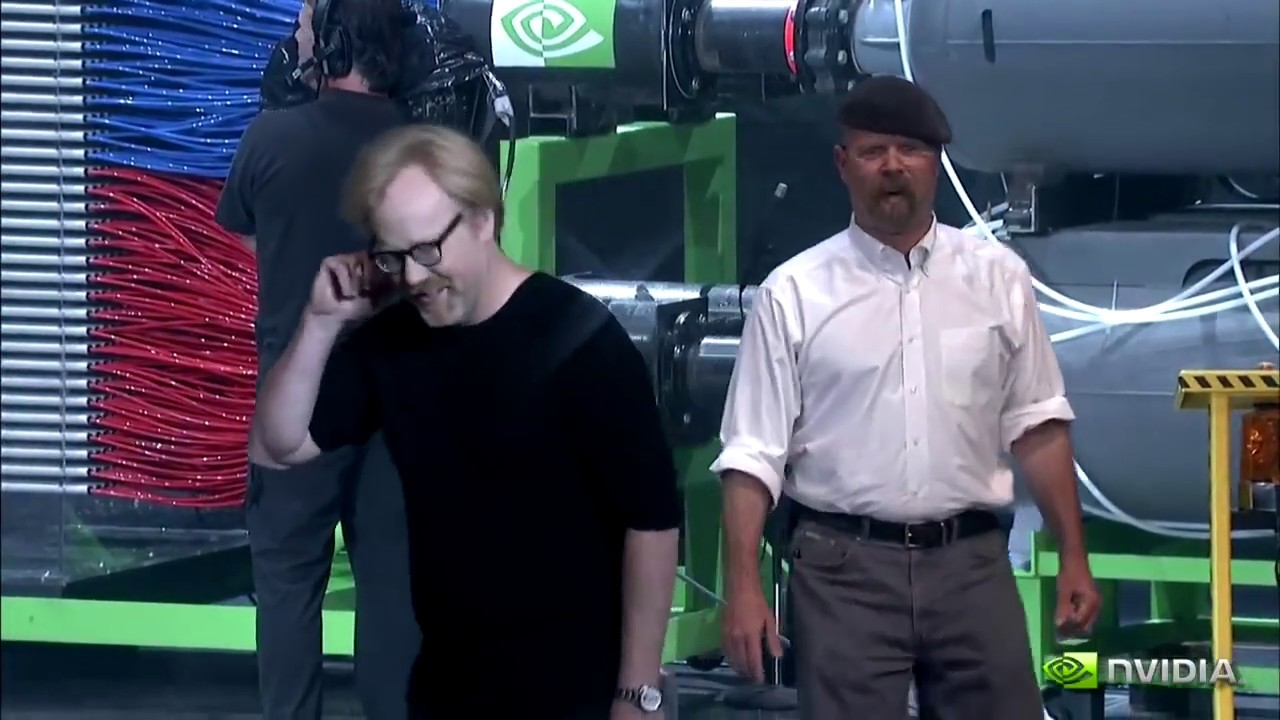
\includegraphics[width=\linewidth,height=4.55cm,keepaspectratio]{mythbusters-gpu-cpu.jpg}}
    \column{.28\textwidth}
    {\large\bfseries CPU vs. GPU\par}
    \vspace{.4cm}
    {\small One paintball at a time.\par}
    \vspace{.3cm}
    {\small Many paintballs together.\par}
    \vspace{.5cm}
    \href{https://www.youtube.com/watch?v=8_ZTvG1WQxM}{\color{work}\small$\blacktriangleright$\; Watch the demo}
  \end{columns}
  \takeaway{Parallel work becomes easy to see when the output is a picture.}
  \credit{https://www.youtube.com/watch?v=8_ZTvG1WQxM}{NVIDIA NVISION 08 / MythBusters demo · video re-upload: HOSTKEY}
  \note{{\small\color{muted}[진행 메모: 시간이 허용되면 사진이나 오른쪽 링크를 눌러 영상을 재생한다. 아래는 읽을 대사.]}

  MythBusters가 2008년 NVIDIA 행사에서 보여준 시연입니다. 한쪽은 페인트볼을 하나씩 쏘고, 다른 쪽은 많은 페인트볼을 함께 쏴서 그림을 만듭니다. 같은 그림을 완성하는 두 방식의 차이에 주목해보시면 됩니다.

  실제 CPU도 병렬로 계산할 수 있고, 어느 방식이 빠른지는 작업에 따라 달라집니다. 이 시연이 잘 보여주는 것은 여러 위치의 작업을 함께 진행하는 모습입니다. 그림을 그리는 일에는 왜 이런 병렬성이 많았을까요?}
\end{frame}

\section{From pictures to programs}
\subsection{Rendering and shaders}
% Source manuscript §1.
\begin{frame}{The original deadline: draw the next frame}
  \blackfiguretop
  \noindent\makebox[\linewidth][c]{%
    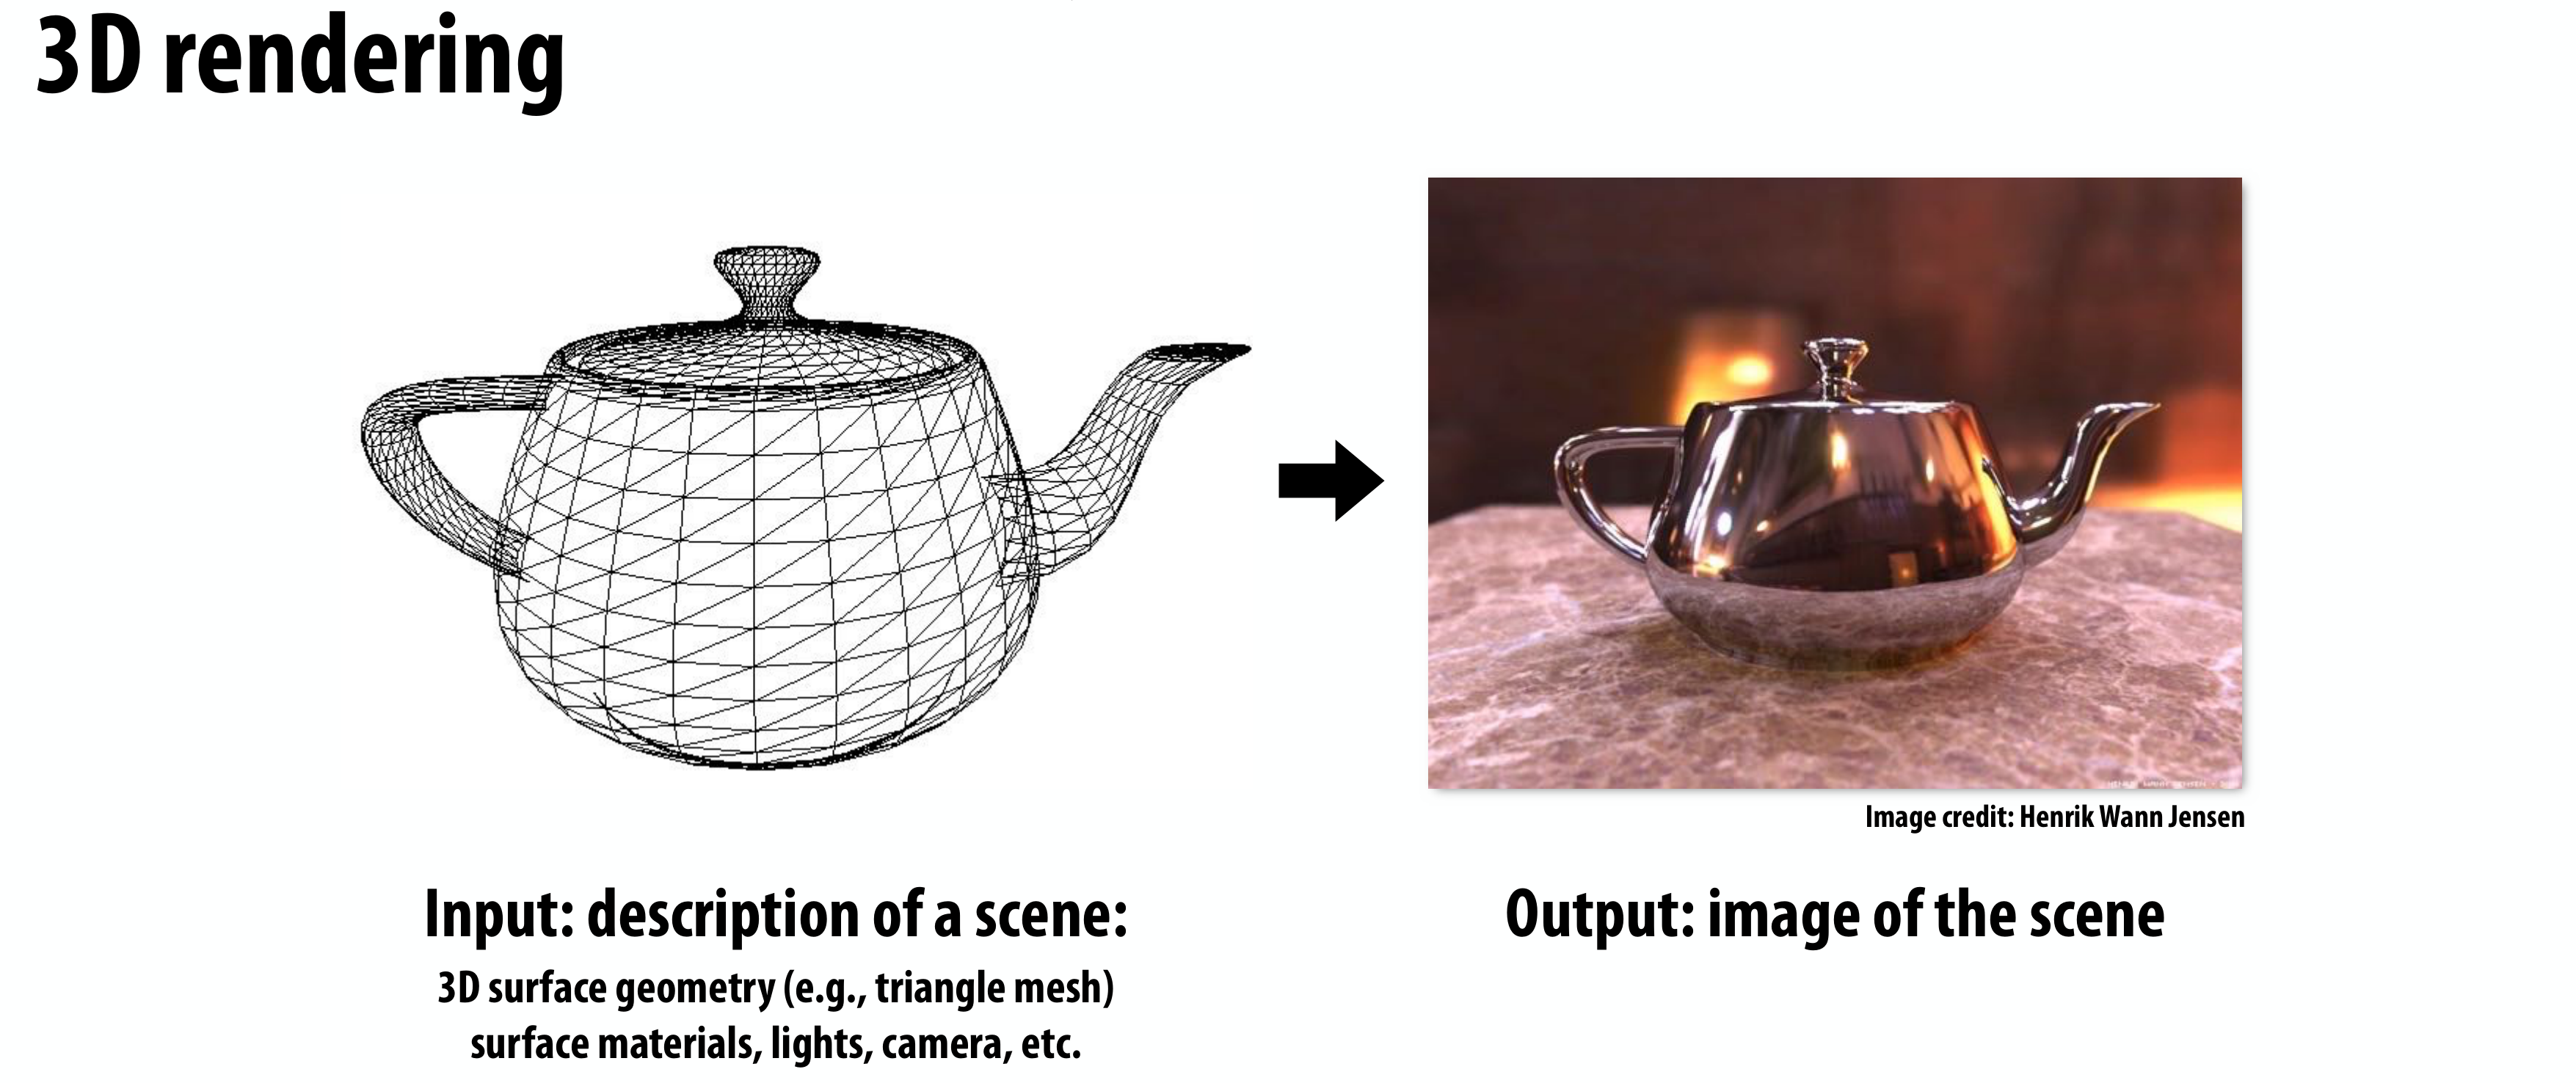
\includegraphics[width=12.8cm,height=4.65cm,keepaspectratio]{stanford-rendering.png}}
  \takeaway{Geometry + materials + lights + camera $\longrightarrow$ an image}
  \credit{https://gfxcourses.stanford.edu/cs149/fall25content/media/gpuarch/07_gpuarch.pdf}{Stanford CS149, Fall 2025 · slide 5 · image: Henrik Wann Jensen}
  \note{게임 속에서 햇빛이 비치는 호숫가를 걷는다고 생각해봅시다. 카메라가 움직이면 화면에 보이는 물결과 가려짐, 반사 모습이 달라집니다. 컴퓨터는 물체의 삼각형들, 재질, 조명, 카메라 위치를 가지고 다음 화면을 계산해야 합니다. 이 작업이 렌더링입니다.

  화면의 주전자도 마찬가지입니다. 왼쪽에는 표면의 모양을 나타내는 기하 정보가 있고, 오른쪽에는 빛과 재질을 반영한 이미지가 있습니다. GPU는 원래 이런 3차원 그래픽을 빠르게 처리하기 위해 발전했습니다. 게임에서는 이 계산을 반복해 다음 장도 정해진 시간 안에 계속 만들어야 합니다.}
\end{frame}

\begin{frame}{Millions of positions. The same kind of calculation.}
  \begin{diagram}{4.3}
    \foreach \x in {0,...,23} \foreach \y in {0,...,11} {
      \pgfmathtruncatemacro{\tint}{15+mod(3*\x+5*\y,65)}
      \fill[work!\tint!white] (\x*.22,\y*.22+.72) rectangle ++(.20,.20);
    }
    \node[lab,anchor=west] at (0,.35) {Different positions, different inputs};
    \node[anchor=west,font=\Large\bfseries] at (6.4,3.35) {1920 $\times$ 1080};
    \node[anchor=west,lab] at (6.4,2.8) {output pixels per frame};
    \node[anchor=west,font=\Large\bfseries] at (6.4,2.05) {$\times\;60$ frames / second};
    \draw[line] (6.4,1.45)--(14.5,1.45);
    \node[anchor=west,font=\Large\bfseries,text=work] at (6.4,.85) {$\approx 124$ million};
    \node[anchor=west,lab] at (6.4,.3) {output pixels per second};
  \end{diagram}
  \takeaway{The opportunity is repeated work across independent data.}
  \note{1920 곱하기 1080 화면에는 약 200만 개의 픽셀이 있습니다. 이것을 초당 60장 만들면 매초 약 1억 2천4백만 개의 출력 픽셀을 만들어야 합니다. 이것은 연산 횟수가 아니라 출력 픽셀 수입니다. 하나의 픽셀을 정하기 위해서는 훨씬 많은 계산이 필요할 수 있습니다.

  여기서 중요한 것은 단순히 숫자가 크다는 사실만이 아닙니다. 수면의 이 지점에서도 빛의 반사를 계산하고, 바로 옆 지점에서도 비슷한 계산을 합니다. 위치와 방향 같은 입력은 다르지만 적용할 계산법은 같을 수 있습니다. 서로 다른 위치에 대해 비슷한 계산을 아주 많이 한다는 성질이 GPU가 활용할 수 있는 병렬성의 출발점입니다.}
\end{frame}

% Source manuscript §2.
\begin{frame}[fragile]{A shader is a program for a graphics stage}
  \vspace{.15cm}
  \begin{columns}[T,onlytextwidth]
    \column{.54\textwidth}
    \kicker{ONE FRAGMENT'S WORK}
\begin{lstlisting}[language={},basicstyle=\ttfamily\fontsize{10.2}{17}\selectfont]
base   = read_surface_color(uv)
light  = max(dot(normal, light_dir), 0)
output = base * light
\end{lstlisting}
    \vspace{.35cm}
    \begin{compactitems}
      \item Programmable behavior replaces a fixed formula.
      \item A fragment is a candidate contribution to a pixel.
    \end{compactitems}
    \column{.40\textwidth}
    \begin{tikzpicture}[x=1cm,y=1cm]
      \node[workbox,minimum width=5.7cm,minimum height=.8cm] (p) at (2.85,3.4)
        {\textbf{One shader program}};
      \foreach \x in {0,...,7} \foreach \y in {0,...,3} {
        \pgfmathtruncatemacro{\tint}{15+7*\x+4*\y}
        \fill[work!\tint!white] (\x*.66+.24,\y*.44+.15) rectangle ++(.59,.37);
      }
      \draw[flow] (p.south)--(2.85,2.1);
      \node[lab] at (2.85,-.25) {Many fragments, many input values};
    \end{tikzpicture}
  \end{columns}
  \takeaway{Write how one surface point is shaded; apply it across the surface.}
  \credit{https://gfxcourses.stanford.edu/cs149/fall25content/media/gpuarch/07_gpuarch.pdf}{Concept: Stanford CS149, Fall 2025 · slides 11–14 · simplified pseudocode}
  \note{한 표면의 여러 위치에는 같은 계산을 반복하지만, 어떤 계산을 반복할지는 소재에 따라 고르고 싶습니다. 물과 벽돌의 표면색을 계산하는 방식은 다를 테니까요. 정해진 기능을 수행하던 그래픽 파이프라인의 일부를 프로그래머가 작성한 코드로 바꿀 수 있게 된 것이 프로그래머블 셰이더입니다. 셰이더는 그래픽 처리의 한 단계에서 실행되는 프로그램입니다.

  삼각형을 화면에 펼치면 화면 위치별로 처리할 조각, 즉 프래그먼트가 생깁니다. 여기에 프래그먼트 셰이더를 적용합니다. 이 조각은 가려짐 검사 등을 거쳐 최종 픽셀에 기여할 수 있는 후보입니다.

  화면의 코드는 표면색을 읽고, 빛을 얼마나 정면으로 받는지 구한 다음, 둘을 곱합니다. 같은 표면의 여러 조각에 이 프로그램을 반복 적용합니다. 계산법은 같아도 위치별 입력이 달라 결과색은 달라집니다.}
\end{frame}

% Source manuscript §3.
\subsection{GPGPU and CUDA}
\begin{frame}{Do those numbers have to be colors?}
  \begin{diagram}{4.4}
    \node[lab,anchor=west] at (0,4.15) {THE GRAPHICS INTERPRETATION};
    \node[membox,minimum width=3.65cm,minimum height=1cm] (colors) at (1.9,3.2)
      {Surface inputs};
    \node[workbox,minimum width=3.65cm,minimum height=1cm] (shader) at (7.35,3.2)
      {\textbf{Shader}};
    \node[membox,minimum width=3.65cm,minimum height=1cm] (image) at (12.8,3.2)
      {Output colors};
    \draw[flow] (colors)--(shader); \draw[flow] (shader)--(image);
    \draw[line] (0,2.2)--(14.7,2.2);
    \node[lab,anchor=west] at (0,1.85) {THE COMPUTE INTERPRETATION};
    \node[membox,minimum width=3.65cm,minimum height=1cm] (values) at (1.9,.9)
      {Scientific data};
    \node[workbox,minimum width=3.65cm,minimum height=1cm] (function) at (7.35,.9)
      {\textbf{Function}};
    \node[membox,minimum width=3.65cm,minimum height=1cm] (result) at (12.8,.9)
      {Output values};
    \draw[flow] (values)--(function); \draw[flow] (function)--(result);
  \end{diagram}
  \takeaway{GPGPU: General-Purpose Computing on GPUs}
  \note{이 구조를 보던 연구자가 이런 생각을 했다고 해봅시다. 저 숫자가 꼭 색깔이어야 할까? GPU는 입력값을 사람이 물의 색이라고 부르는지, 온도라고 부르는지 신경 쓰지 않습니다. 숫자를 읽고 계산한 다음 결과를 저장할 뿐입니다.

  위쪽은 그래픽의 언어입니다. 각 위치의 입력을 셰이더에 넣어 출력색을 만듭니다. 아래쪽에서는 이름만 바꿨습니다. 각 데이터 포인트의 입력을 함수에 넣어 결과값을 만듭니다. 기존 기계를 새로 발명한 것이 아니라, 원래 하던 일에서 그림이라는 의미를 벗겨낸 것입니다. 이런 식으로 많은 데이터에 같은 계산을 병렬로 적용할 수 있다면 그래픽이 아니어도 GPU를 활용할 수 있습니다. 이것이 초기 GPGPU의 핵심 관점입니다.}
\end{frame}

% Source manuscript §4.
\begin{frame}{To add two arrays, first draw two triangles}
  \begin{diagram}{4.5}
    \node[anchor=west,font=\large\ttfamily] at (0,4.15) {C[i] = A[i] + B[i]};
    \node[membox,minimum width=2.65cm,minimum height=.7cm] (a) at (1.4,2.85) {Texture A};
    \node[membox,minimum width=2.65cm,minimum height=.7cm] (b) at (1.4,1.5) {Texture B};
    \fill[workLight] (4.1,.55) rectangle (7.65,4.1);
    \fill[work!14] (4.1,.55)--(7.65,4.1)--(7.65,.55)--cycle;
    \draw[step=.44375cm,workBorder,very thin] (4.1,.55) grid (7.65,4.1);
    \draw[work,line width=1pt] (4.1,.55) rectangle (7.65,4.1);
    \draw[work,line width=1pt] (4.1,.55)--(7.65,4.1);
    \draw[flow] (a.east)--(4.0,2.85); \draw[flow] (b.east)--(4.0,1.5);
    \node[lab] at (5.875,.2) {512 $\times$ 512 output positions};
    \node[anchor=west,text width=5.3cm,font=\small,align=left] at (9,3.25)
      {\textbf{1}\quad Set the output image size.\\[.5em]
       \textbf{2}\quad Cover it with two triangles.\\[.5em]
       \textbf{3}\quad Add values in a fragment shader.};
    \node[anchor=west,font=\small,text=mem] at (9,1.0) {Interpret the output as an array.};
    \draw[flow] (7.8,2.3)--(8.65,2.3);
  \end{diagram}
  \takeaway{A draw call to the GPU; an array operation to the researcher.}
  \credit{https://gfxcourses.stanford.edu/cs149/fall25content/media/gpuarch/07_gpuarch.pdf}{Redrawn from Stanford CS149, Fall 2025 · slide 17}
  \note{발견과 실제 사용 사이에는 재미있는 장애물이 있었습니다. 우리가 하고 싶은 것은 A와 B의 같은 원소를 더해서 C에 쓰는 것뿐인데, GPU에 일을 시키는 통로가 그래픽 API였습니다. 그래서 계산을 그림 그리기로 번역해야 했습니다.

  512 곱하기 512개의 원소를 처리하려면 먼저 출력 이미지 크기를 그렇게 설정합니다. 입력 배열은 원래 표면의 무늬를 저장하던 텍스처에 넣습니다. 그다음 출력 영역을 정확히 덮는 삼각형 두 개를 그립니다. 그러면 각 위치에 프래그먼트 셰이더가 실행되고, 셰이더는 색을 만드는 대신 A와 B의 값을 읽어 더합니다. 출력된 이미지를 숫자 배열로 해석하면 계산이 끝납니다. GPU에게는 사각형을 그리는 작업이었지만, 연구자에게는 배열 전체에 함수를 적용하는 작업이었던 것입니다.}
\end{frame}

\begin{frame}{“All this just to do A + B”}
  \begin{diagram}{2.5}
    \foreach \x/\name/\label in {1.7/a/{Array as texture},5.45/b/{Draw command},9.2/c/{Fragment shader},13.0/d/{Image output}} {
      \node[plainbox,minimum width=3.1cm,minimum height=1.15cm,font=\small] (\name) at (\x,1.4) {\label};
    }
    \draw[flow] (a)--(b); \draw[flow] (b)--(c); \draw[flow] (c)--(d);
  \end{diagram}
  \begin{itemize}
    \item The entry point still speaks graphics.
    \item Fragment programs have restricted output locations.
    \item Sharing data between executions is constrained.
  \end{itemize}
  \credit{https://web.stanford.edu/class/ee380/Abstracts/061129-SU-EE380-Cuda.pdf}{Ian Buck / NVIDIA · Stanford EE380, November 2006 · slides 7–8}
  \note{NVIDIA의 2006년 자료도 이 상황을 고작 A 더하기 B를 하려고 이 모든 것을 한다고 표현했습니다. 불편함은 코드가 길어진다는 데서 끝나지 않았습니다.

  지금 본 초기 프래그먼트 경로에서는 결과가 그 조각에 대응하는 그래픽 출력 위치로 나갔습니다. 일반 배열의 원하는 원소에 결과를 쓰거나, 다른 실행의 중간값을 주고받는 계산을 표현하는 데 제약이 있었습니다. 입구부터 내부 규칙까지 그림을 그리는 장치에 맞춰져 있었던 것입니다. 그렇다면 이 우회 경로를 정식 계산 인터페이스로 바꿀 수 있지 않을까요?}
\end{frame}

% Source manuscript §5. Dates refer to architecture announcement / Toolkit.
\begin{frame}{CUDA made compute a first-class interface}
  \begin{diagram}{4.55}
    \node[anchor=north west,inner sep=0] at (0,4.35)
      {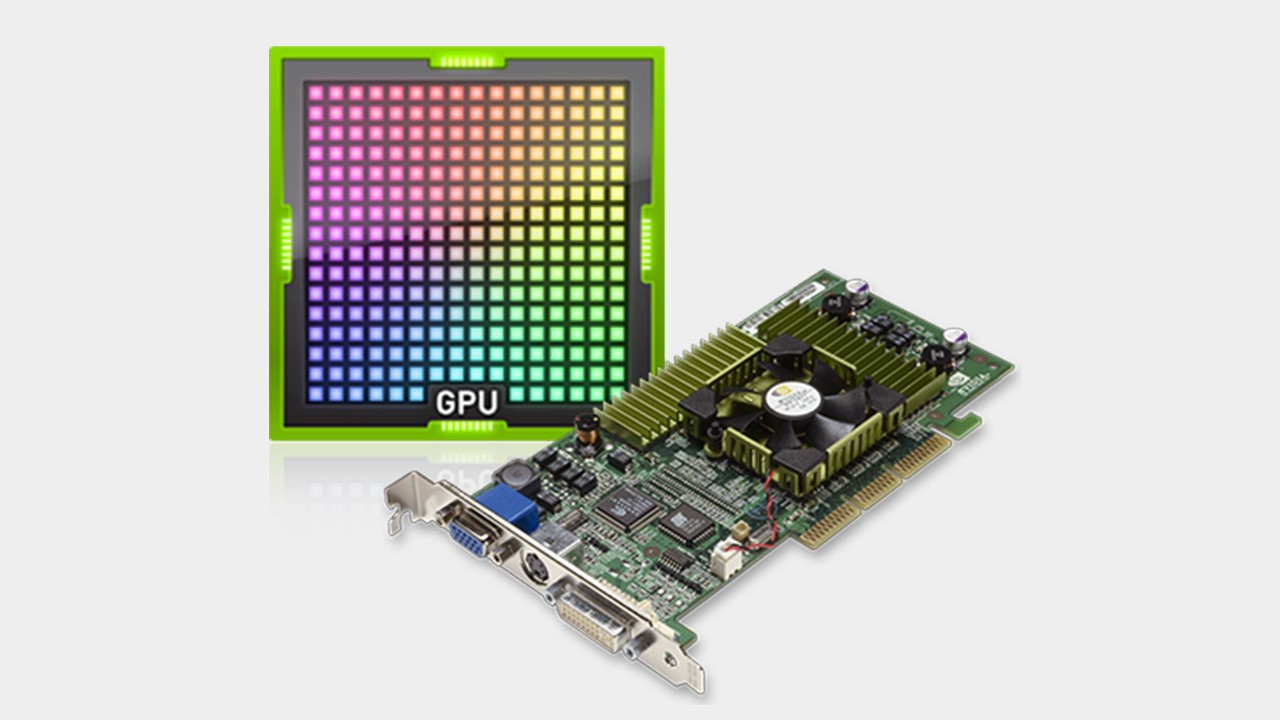
\includegraphics[width=4.5cm]{nvidia-1999-gpu.jpeg}};
    \node[anchor=north west,inner sep=0] at (5.1,4.35)
      {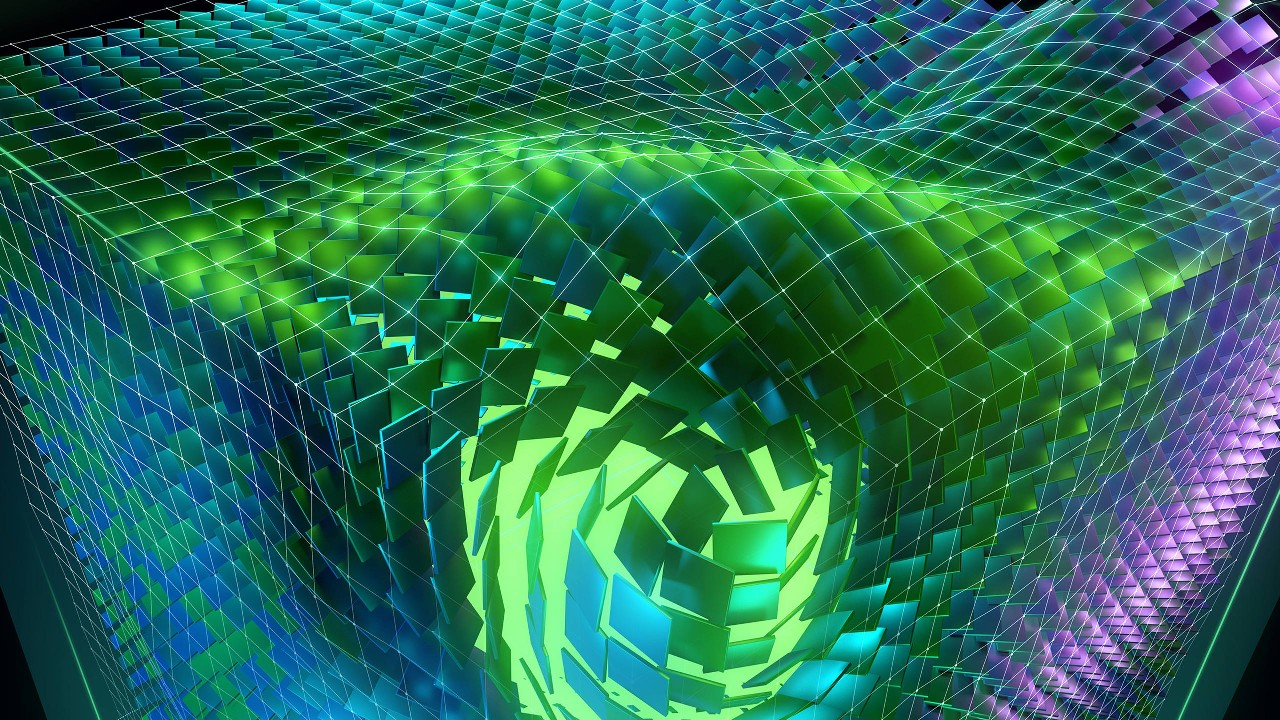
\includegraphics[width=4.5cm]{nvidia-2006-cuda.jpeg}};
    \node[plainbox,minimum width=4.5cm,minimum height=2.53cm] at (12.45,3.085)
      {{\fontsize{20}{26}\selectfont\ttfamily launch()}\\[.3cm]{\small CUDA Toolkit 1.0}};
    \draw[line,line width=1pt] (0,1.4)--(14.7,1.4);
    \foreach \x/\year/\label in {0/1999/{GeForce 256},5.1/2006/{CUDA architecture},10.2/2007/{CUDA Toolkit 1.0}} {
      \fill[hw] (\x+.1,1.4) circle (.055);
      \node[anchor=west,font=\large\bfseries] at (\x,.9) {\year};
      \node[anchor=west,lab] at (\x,.37) {\label};
    }
  \end{diagram}
  \takeaway{Allocate buffers. Run a kernel. Read and write data directly.}
  \credit{https://www.nvidia.com/en-us/about-nvidia/corporate-timeline/}{Images / 2006: NVIDIA corporate timeline · Toolkit 1.0: NVIDIA guide, June 2007}
  \note{이 변화를 연표로 정리해보겠습니다. 왼쪽의 1999년 GeForce 256은 그래픽 GPU의 이정표입니다. 여기서 계산 플랫폼으로 넘어가는 핵심 전환은 가운데와 오른쪽입니다. NVIDIA는 2006년에 CUDA 아키텍처를 공개했고, 2007년에는 CUDA Toolkit 1.0을 출시했습니다.

  이제 GPU 메모리에 일반 배열 버퍼를 준비하고, 그 주소를 사용해 원하는 원소를 읽거나 결과를 쓸 수 있습니다. GPU에서 실행할 프로그램을 커널이라고 하고, 그 실행을 요청하는 것을 launch라고 부릅니다. 삼각형을 그리는 절차 없이 계산을 직접 요청하는 것입니다. 정해진 범위에서 실행끼리 데이터를 공유하고 동기화하는 기능도 제공합니다. 계산을 시키는 입구와 가능한 동작이 함께 바뀐 것입니다.}
\end{frame}

\begin{frame}{“Run this program many times.”}
  \begin{diagram}{4.3}
    \node[anchor=west,font=\scriptsize\bfseries,text=muted] at (0,3.9) {THE REQUEST};
    \node[workbox,minimum width=5cm,minimum height=1.4cm,font=\large] (kernel) at (2.55,2.5)
      {\textbf{One program}\\[.12cm]{\small + a collection of inputs}};
    \draw[flow] (kernel.east)--(6.55,2.5);
    \node[hwbox,minimum width=7.65cm,minimum height=2.85cm] (gpu) at (10.5,2.5) {};
    \node[anchor=west,font=\small\bfseries,text=hw] at (7,3.5) {GPU};
    \foreach \x in {0,...,11} \foreach \y in {0,...,2} {
      \draw[workbox,inner sep=0] (7.1+\x*.57,1.55+\y*.48) rectangle ++(.4,.32);
    }
    \node[lab] at (10.5,.55) {Many logical executions};
    \node[lab,anchor=west] at (0,.55) {The data-parallel structure survives.};
  \end{diagram}
  \takeaway{Now look inside the machine that accepts that request.}
  \note{사용자가 이제 하고 싶은 말은 이 프로그램을 많이 실행해달라는 것입니다. 화면을 설정하고 삼각형을 그리라는 말 대신, 실행할 프로그램과 데이터를 직접 건넵니다. 그래픽이라는 외피를 벗겨도 많은 데이터에 같은 계산을 적용한다는 성격은 그대로 남아 있습니다.

  여기서 연대기를 마치고 설계 관점으로 바꿔보겠습니다. 이어지는 설명은 실제 발명 순서를 재현하는 것이 아니라, 이런 요청을 처리할 계산기를 만든다면 어떤 구조가 필요할지 생각해보는 과정입니다.}
\end{frame}

\section{The execution engine}
\subsection{Warps and SIMT}
% Source manuscript §6.
\begin{frame}{A warp groups 32 logical threads}
  \begin{diagram}{4.5}
    \node[workbox,minimum width=5cm,minimum height=.65cm] (inst) at (7.4,4.02)
      {One instruction: \texttt{ADD}};
    \draw[flow] (inst.south)--(7.4,3.25);
    \foreach \i in {0,...,31} {
      \pgfmathtruncatemacro{\col}{mod(\i,16)}
      \pgfmathtruncatemacro{\row}{int(\i/16)}
      \node[workbox,minimum width=.75cm,minimum height=.55cm,inner sep=0pt,font=\scriptsize]
        at (.63+\col*.9,2.78-\row*.86) {\i};
    }
    \node[lab,anchor=west] at (.2,1.05) {Thread 0: \texttt{a[0] + b[0]}};
    \node[lab] at (7.4,1.05) {$\cdots$};
    \node[lab,anchor=east] at (14.6,1.05) {Thread 31: \texttt{a[31] + b[31]}};
    \node[anchor=west,font=\small] at (.2,.25)
      {\textbf{SIMT}\quad Single Instruction, Multiple Threads};
  \end{diagram}
  \takeaway{A warp describes grouped execution; it is not a 32-core component.}
  \credit{https://docs.nvidia.com/cuda/cuda-programming-guide/01-introduction/programming-model.html}{NVIDIA CUDA Programming Guide · Warps and SIMT}
  \note{여러 데이터에 대해 덧셈을 해야 한다고 해봅시다. 각 계산의 입력은 다르지만, 지금 해야 할 명령은 모두 덧셈입니다. 하나의 명령으로 여러 데이터의 계산을 함께 진행하면 명령을 전달하고 제어하는 비용을 나눌 수 있습니다.

  프로그램의 개별 실행을 thread라고 합니다. NVIDIA CUDA GPU가 이 실행들을 함께 관리하는 warp의 폭은 32입니다. 프로그램에서 정하는 더 큰 작업 묶음인 block 안에서, 연속된 번호의 thread를 32개씩 묶습니다. block을 어떻게 구성하는지는 뒤의 코드 예제에서 보겠습니다.

  파란 상자는 논리적인 실행을 나타냅니다. warp가 물리적 연산기 32개로 된 부품이거나 thread가 연산기 하나를 영구적으로 차지한다는 뜻은 아닙니다. 프로그래머는 thread마다 할 일을 쓰고, 하드웨어는 같은 명령을 묶어 처리합니다. 이것이 SIMT, Single Instruction, Multiple Threads입니다.}
\end{frame}

\begin{frame}{Same program does not always mean the same path}
  \begin{diagram}{4.4}
    \node[anchor=west,font=\small\ttfamily] at (0,4.05)
      {if (lane < 16) \{ path\_A(); \} else \{ path\_B(); \}};
    \node[lab,anchor=west] at (0,3.2) {Lane};
    \foreach \i in {0,...,31} {
      \node[font=\fontsize{6.5}{8}\selectfont,text=muted] at (2.55+\i*.38,3.2) {\i};
      \ifnum\i<16
        \fill[work] (2.38+\i*.38,2.12) rectangle ++(.33,.49);
        \fill[blackPrimary!8] (2.38+\i*.38,1.05) rectangle ++(.33,.49);
      \else
        \fill[blackPrimary!8] (2.38+\i*.38,2.12) rectangle ++(.33,.49);
        \fill[work] (2.38+\i*.38,1.05) rectangle ++(.33,.49);
      \fi
    }
    \node[anchor=west,font=\small\bfseries] at (0,2.36) {Path A};
    \node[anchor=west,font=\small\bfseries] at (0,1.29) {Path B};
    \fill[work] (2.4,.25) rectangle ++(.25,.25);
    \node[lab,anchor=west] at (2.85,.375) {active};
    \fill[blackPrimary!8] (5.1,.25) rectangle ++(.25,.25);
    \node[lab,anchor=west] at (5.55,.375) {masked for this path};
  \end{diagram}
  \takeaway{Divergent paths are processed with different active threads.}
  \credit{https://docs.nvidia.com/cuda/cuda-programming-guide/01-introduction/programming-model.html}{NVIDIA CUDA Programming Guide · Warps and SIMT · conceptual mask illustration}
  \note{{\small\color{muted}[보충 메모: Volta 이후의 Independent Thread Scheduling은 thread별 실행 상태를 지원한다. 이 그림은 경로별 참여 관계를 설명하며 실제 명령 발행 순서를 정하지 않는다.]}

  warp 안에서 0번부터 31번까지의 논리적인 thread 자리를 lane이라고 부릅니다. 화면의 조건문은 lane 번호가 16보다 작은 thread를 A 경로로, 나머지를 B 경로로 보냅니다. 같은 프로그램을 실행해도 입력이나 조건에 따라 이렇게 경로가 갈릴 수 있습니다.

  A 경로의 명령에는 앞의 16개 thread가 참여하고, B 경로의 명령에는 뒤의 16개가 참여합니다. 파란 칸이 각 경로의 활성 thread이며, 이 그림은 정확한 사이클표가 아닙니다. 이것이 warp divergence입니다. 같은 warp 안에서 실행 경로가 비슷하면 한 명령에 함께 참여할 thread가 많아져 자원을 효율적으로 활용하기 쉽습니다.}
\end{frame}

% Source manuscript §7. Explicitly a design thought experiment.
\subsection{SMs and GPU organization}
\begin{frame}{Arithmetic needs state, and state has to live somewhere}
  \begin{diagram}{4.4}
    \node[lab,anchor=west] at (0,4.15) {A DESIGN THOUGHT EXPERIMENT};
    \node[membox,minimum width=3.45cm,minimum height=1.5cm] (state) at (1.8,2.7)
      {\textbf{Intermediate values}\\[.12cm]{\small + execution state}};
    \node[hwbox,minimum width=3.45cm,minimum height=1.5cm] (alu) at (12.85,2.7)
      {\textbf{Arithmetic units}\\[.12cm]{\small somewhere on the chip}};
    \draw[flow,draw=mem] (state.east) to[bend left=12]
      node[above,lab,text=mem] {operands must travel too} (alu.west);
    \draw[flow,draw=mem] (alu.west) to[bend left=12]
      node[below,lab,text=mem] {results must be kept for later} (state.east);
    \draw[line] (0,1.25)--(14.7,1.25);
    \node[anchor=west,font=\small] at (0,.65)
      {Store values.\qquad Track progress.\qquad Choose the next instruction.};
  \end{diagram}
  \takeaway{Adding execution units also creates a data-movement problem.}
  \note{경로가 갈리는 경우까지 보았으니, 이제 이 warp들을 실제로 처리할 기계를 생각해봅시다. 연산기를 칩 안에 잔뜩 넣으면 충분할까요? 프로그램은 덧셈 한 번으로 끝나지 않습니다. 값을 읽고, 곱하고, 더하고, 조건을 검사하려면 중간값과 실행 상태를 기억할 자리, 다음 명령을 고르는 장치도 있어야 합니다.

  모든 warp를 한곳에서 관리하고 칩 전체의 빈 연산기로 보내는 구조를 상상해봅시다. 값은 왼쪽에 있고 빈 연산기는 오른쪽에 있다면 필요한 값도 이동해야 합니다. 결과를 다시 가져오거나 멀리서 접근할 연결망도 필요합니다. 연산기를 늘릴 때에는 계산에 필요한 상태를 어디에 두고 어떻게 옮길지도 함께 설계해야 합니다.}
\end{frame}

% Source manuscript §8.
\begin{frame}{An SM keeps execution and its working state close}
  \begin{diagram}{4.65}
    \draw[hwbox] (0,.08) rectangle (10.15,4.6);
    \node[anchor=west,font=\small\bfseries,text=hw] at (.28,4.27)
      {SM · Streaming Multiprocessor};
    \node[workbox,minimum width=3.3cm,minimum height=.8cm,font=\small] (resident) at (2.05,3.35)
      {Resident warps};
    \node[hwbox,minimum width=5.5cm,minimum height=.8cm,font=\small] (scheduler) at (6.9,3.35)
      {Warp schedulers};
    \draw[flow] (resident.east)--(scheduler.west);
    \node[membox,minimum width=9.35cm,minimum height=.6cm,font=\small] (registers) at (5.07,2.4)
      {Registers · values for resident threads};
    \node[hwbox,minimum width=4.5cm,minimum height=.7cm,font=\small] (math) at (2.7,1.47)
      {Arithmetic units};
    \node[hwbox,minimum width=4.5cm,minimum height=.7cm,font=\small] (lsu) at (7.47,1.47)
      {Load / store units};
    \node[membox,minimum width=9.35cm,minimum height=.55cm,font=\small] at (5.07,.56)
      {Shared memory / L1 cache};
    \node[anchor=north west,text width=3.9cm,font=\small,align=left] at (10.8,4.1)
      {\textbf{Manage many warps.}\\[.22cm]
       Keep their state nearby.\\[.38cm]
       Feed ready instructions to execution units.};
    \node[anchor=south west,lab,text width=3.85cm,align=left] at (10.8,.25)
      {Conceptual organization.\\Internal partitions vary by architecture.};
  \end{diagram}
  \takeaway{Warp = grouped work.\qquad SM = the hardware that executes it.}
  \credit{https://docs.nvidia.com/cuda/cuda-programming-guide/01-introduction/programming-model.html}{NVIDIA CUDA Programming Guide · GPU Hardware Model · original schematic}
  \note{그렇다면 서로 자주 주고받는 것들을 가까이 묶어봅시다. 연산기 옆에 각 thread의 현재 작업값을 보관할 레지스터를 두고, 실행을 관리할 스케줄러와 메모리 읽기·쓰기 장치도 함께 둡니다. NVIDIA GPU에서 이런 역할을 하는 단위가 SM, Streaming Multiprocessor입니다. 아래쪽 shared memory와 L1 캐시는 SM 가까이에서 데이터를 사용할 수 있게 해주는 저장 자원입니다.

  이 SM에 실행 상태와 자원을 배정받아 머무는 warp를 resident warp라고 합니다. SM은 여러 warp의 상태를 보관하고, 스케줄러는 그중 입력값과 실행 자원이 준비된 명령을 골라 발행합니다. 머무는 warp 수와 한순간에 명령을 처리하는 연산기 수는 다른 숫자입니다.

  실제 SM의 내부 구획은 아키텍처에 따라 달라지며, 여기서는 여러 스케줄러와 자원을 묶어 그렸습니다. 핵심은 하나의 SM이 여러 warp의 상태를 가까이 두고 실행을 진행시킨다는 것입니다.}
\end{frame}

% Source manuscript §9.
\begin{frame}{Scale the GPU by repeating that execution engine}
  \begin{diagram}{4.5}
    \draw[hwbox] (0,.15) rectangle (11.1,4.45);
    \node[anchor=west,font=\small\bfseries,text=hw] at (.3,4.1) {GPU chip · simplified compute view};
    \foreach \x in {0,...,3} \foreach \y in {0,...,1} {
      \pgfmathtruncatemacro{\id}{\x+4*\y}
      \node[hwbox,minimum width=2.35cm,minimum height=.82cm,font=\small] at (1.52+\x*2.67,3.22-\y*1.15)
        {\textbf{SM \id}};
    }
    \foreach \x in {0,...,3} {
      \draw[line] (1.52+\x*2.67,1.64)--(1.52+\x*2.67,1.3);
    }
    \node[membox,minimum width=10.1cm,minimum height=.6cm,font=\small] (l2) at (5.54,.98)
      {GPU-wide L2 cache + memory system};
    \node[membox,minimum width=2.8cm,minimum height=2.35cm,font=\small] (vram) at (13.1,2.4)
      {\textbf{GPU memory}\\[.2cm]VRAM\\[.13cm]{\scriptsize e.g., GDDR / HBM}};
    \draw[flow,<->] (11.12,2.4)--(vram.west);
  \end{diagram}
  \takeaway{Share control within a warp; keep execution resources local to an SM.}
  \credit{https://docs.nvidia.com/cuda/cuda-programming-guide/01-introduction/programming-model.html}{NVIDIA CUDA Programming Guide · GPU Hardware Model · illustrative SM count}
  \note{이제 자기 몫의 실행을 관리할 수 있는 SM을 여러 개 배치해 GPU를 키워봅시다. 각 SM은 가까운 레지스터와 실행 자원을 사용합니다. 그 바깥에는 여러 SM이 함께 사용하는 L2 캐시와 메모리 시스템이 연결되고, 오른쪽의 큰 GPU 메모리인 VRAM에는 텐서 같은 입력과 출력을 담습니다.

  warp에서는 같은 명령의 제어를 함께 쓰고, SM마다 실행 상태와 연산 자원을 가까이 묶습니다. 그런 SM을 반복해서 배치하면 각각 자기 몫의 일을 진행할 수 있습니다. 실제 GPU의 전체 부품을 그린 것은 아니지만, 범용 계산을 담당하는 중심 구조를 이렇게 볼 수 있습니다. 이제 실제 칩의 예시와 연결해보겠습니다.}
\end{frame}

\begin{frame}{A concrete example: the NVIDIA V100}
  \blackfiguretop
  \begin{columns}[c,onlytextwidth]
    \column{.54\textwidth}
    \centering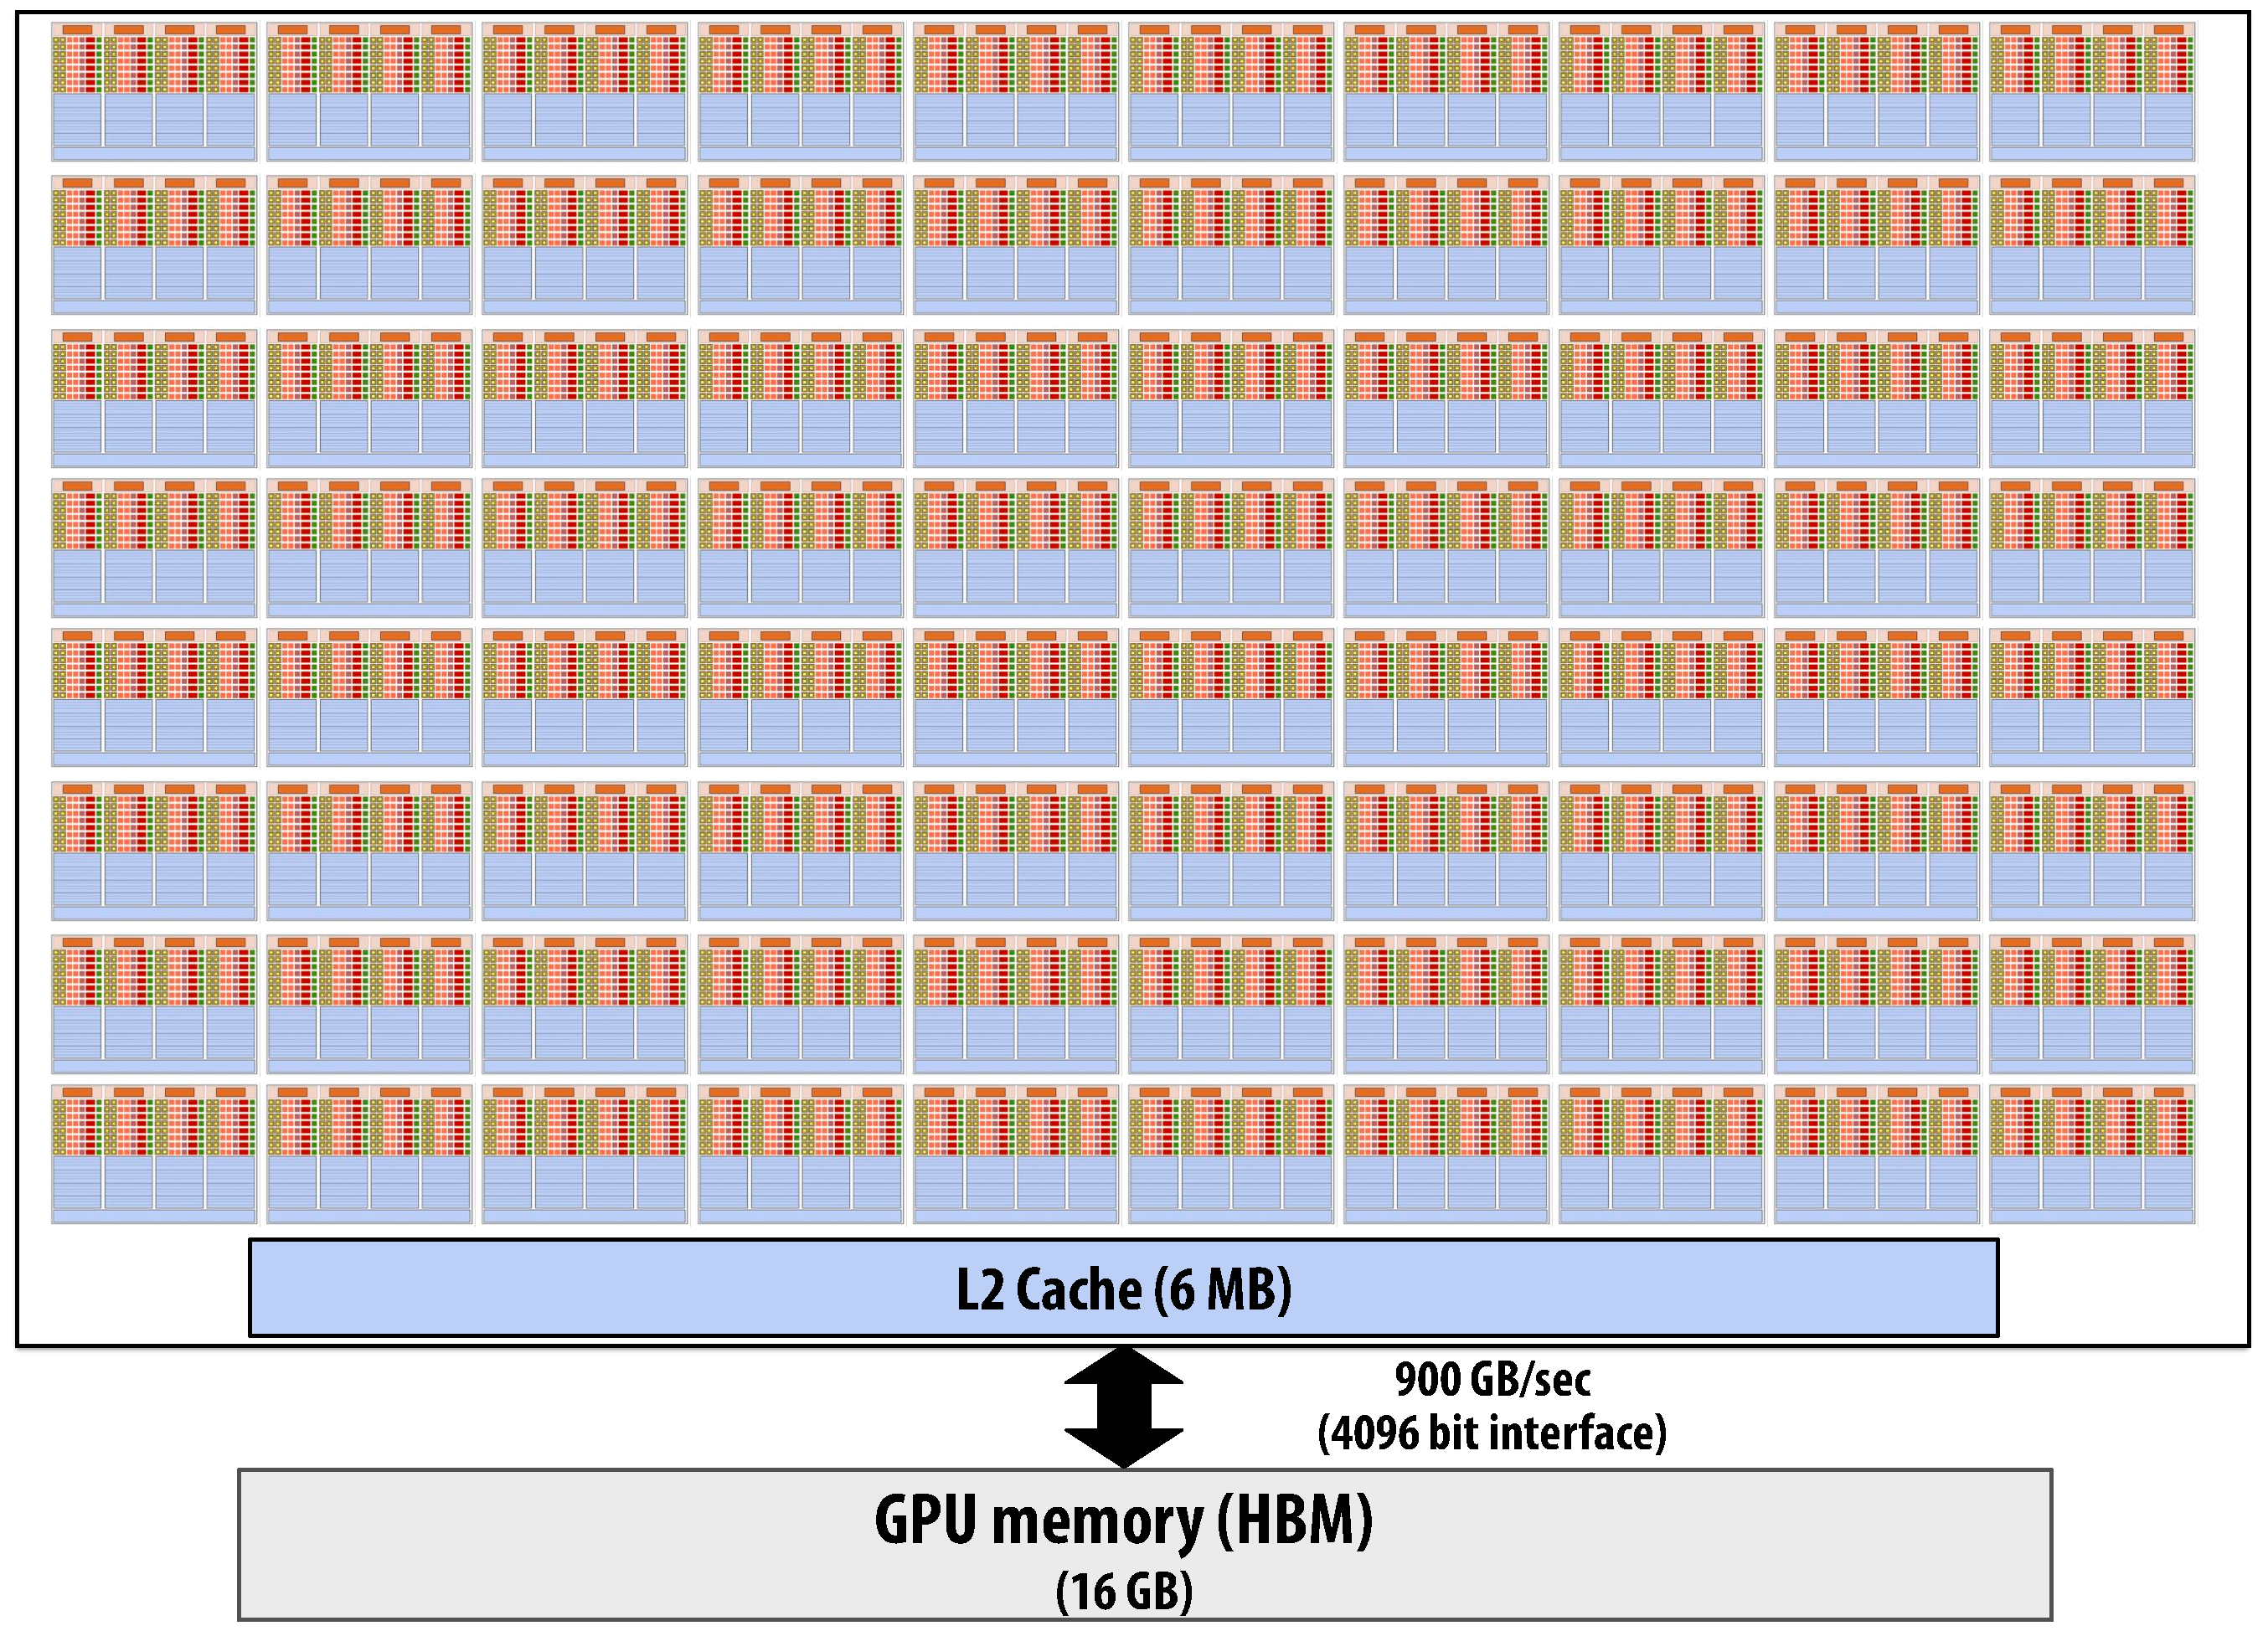
\includegraphics[width=7.45cm,height=5.4cm,keepaspectratio]{stanford-v100-complete.pdf}
    \column{.39\textwidth}
    {\fontsize{26}{30}\selectfont\bfseries\color{hw}80 SMs\par}
    \vspace{.2cm}
    {\small Repeated execution engines\par}
    \vspace{.5cm}
    {\large\bfseries Shared L2 cache\par}
    \vspace{.15cm}
    {\small A cache shared by the SMs\par}
    \vspace{.5cm}
    {\large\bfseries HBM2 memory\par}
    \vspace{.15cm}
    {\small Stores the inputs and outputs\par}
    \vspace{.45cm}
    {\scriptsize\color{muted}Historical example, not a universal GPU specification.}
  \end{columns}
  \credit{https://gfxcourses.stanford.edu/cs149/fall25content/media/gpuarch/07_gpuarch.pdf}{Stanford CS149, Fall 2025 · slide 52 · V100 configuration shown in the lecture}
  \note{{\small\color{muted}[진행 메모: 왼쪽 그림 맨 위 줄의 맨 왼쪽 회색 직사각형 전체를 가리킨다. 내부의 네 세로 구획을 합친 묶음이 SM 하나다.]}

  Stanford 강의에 나온 NVIDIA V100의 사례입니다. 원본 자료의 색을 그대로 쓴 그림이라 앞의 도식과 색 의미가 다릅니다. 맨 위 줄의 맨 왼쪽을 보면, 주황색 막대 네 개와 그 아래 색 칸들을 함께 감싼 회색 직사각형이 있습니다. 이 묶음 전체가 SM 하나이고, 이 V100 구성에는 이런 SM이 80개 있습니다.

  아래의 긴 상자는 여러 SM이 함께 사용하는 L2 캐시입니다. 그 바깥의 HBM2 메모리는 큰 입력과 출력을 저장합니다. 세대마다 개수와 구성은 달라져도, 여러 실행 엔진이 메모리 시스템에 연결된다는 구조를 확인할 수 있습니다. 그러면 이 여러 SM에 일을 나누는 것은 누구의 몫일까요?}
\end{frame}

% Source manuscript §10–11.
\section{Following A + B}
\subsection{From tensors to threads}
\begin{frame}{Describe the work; the GPU places it}
  \begin{diagram}{4.2}
    \node[workbox,minimum width=5.7cm,minimum height=2.1cm] (request) at (2.95,2.5)
      {\textbf{The programmer specifies}\\[.25cm]
       {\small What each execution does}\\[.16cm]
       {\small How many executions to launch}};
    \node[hwbox,minimum width=5.7cm,minimum height=2.1cm] (machine) at (11.75,2.5)
      {\textbf{The GPU manages}\\[.25cm]
       {\small Placement on available SMs}\\[.16cm]
       {\small Instruction issue within each SM}};
    \draw[flow] (request)--node[above,lab] {launch} (machine);
    \node[lab,anchor=west] at (0,.65)
      {PyTorch chooses CUDA implementations underneath tensor operations.};
  \end{diagram}
  \takeaway{A work description is not a physical placement plan.}
  \note{이제 사용자의 입장에서 보면, CUDA 프로그래머의 몫은 할 일의 구성을 표현하는 것입니다. 각 실행이 무엇을 할지, 그 실행들을 어떻게 묶어서 얼마나 실행할지 정합니다. 어느 SM이 그 일을 맡을지는 GPU가 사용 가능한 자원에 맞춰 결정하고, 각 SM이 명령을 실행합니다.

  PyTorch를 쓰면 커널을 고르고 실행 규모를 정하는 과정도 프레임워크가 맡습니다. 우리는 텐서에 대한 연산을 요청합니다. 다음 코드의 한 줄에서 시작해, 그 요청이 방금 본 SM과 warp에 어떻게 도착하는지 따라가보겠습니다.}
\end{frame}

\begin{frame}[fragile]{Start with one line of PyTorch}
  \vspace{.05cm}
\begin{lstlisting}[language=Python,basicstyle=\ttfamily\fontsize{10}{15}\selectfont]
import torch
A = torch.randn(1024, 1024, device="cuda")
B = torch.randn(1024, 1024, device="cuda")
C = A + B
\end{lstlisting}
  \begin{tikzpicture}[x=1cm,y=1cm]
    \path[use as bounding box] (0,0) rectangle (14.8,2.0);
    \foreach \x/\letter in {0/A,5.4/B,10.8/C} {
      \node[anchor=west,font=\small\bfseries,text=mem] at (\x,1.7) {\letter};
      \foreach \i in {0,...,3} \foreach \j in {0,...,1} {
        \draw[memBorder,fill=memLight] (\x+\i*.9,\j*.55) rectangle ++(.82,.47);
      }
      \fill[work] (\x+.9,.55) rectangle ++(.82,.47);
      \node[font=\scriptsize,text=white] at (\x+1.31,.785) {$i$};
    }
    \node[font=\Large] at (4.5,.62) {$+$};
    \node[font=\Large] at (9.9,.62) {$=$};
  \end{tikzpicture}
  \takeaway{Each output needs only its own two inputs. No neighbor must finish first.}
  \note{GPU에 있는 1024 곱하기 1024 행렬 두 개를 더하는 코드입니다. C는 A와 B의 같은 위치에 있는 원소끼리 더한 결과입니다. 행렬 전체를 하나의 숫자로 합치는 연산이 아니라, 같은 크기의 행렬을 만드는 원소별 덧셈입니다.

  여기서 첫 번째 덧셈이 끝나야 두 번째 덧셈을 할 수 있을까요? 그렇지 않습니다. 각 결과에 필요한 것은 자기 위치의 입력 두 개뿐이고, 옆 원소의 결과를 기다릴 필요가 없습니다. 따라서 백만 개가 넘는 덧셈을 여러 실행에 나눠 맡길 수 있습니다. 처음에 보았던 많은 데이터에 같은 계산을 반복하는 구조입니다. 이 계산을 실행하기 전에, 먼저 입력이 어디에 준비되는지 확인하겠습니다.}
\end{frame}

% Source: gpu-101.md, sections 12--15. Educational one-element-per-thread kernel.
% Optional host input path. Insert directly after the first PyTorch code frame.
\begin{frame}[fragile]{If the input starts in CPU memory, copy it to the GPU}
  \begin{diagram}{3.25}
    \node[lab,anchor=west] at (.35,2.95) {HOST};
    \node[lab,anchor=west] at (9.8,2.95) {DEVICE};
    \node[membox,minimum width=4.25cm,minimum height=1.85cm,font=\small] (hostmem) at (2.5,1.72) {\textbf{CPU RAM}\\[6pt]\texttt{A\_cpu}\\Input tensor storage};
    \node[membox,minimum width=4.25cm,minimum height=1.85cm,font=\small] (devmem) at (11.9,1.72) {\textbf{GPU global memory}\\[6pt]\texttt{A}\\Buffer in VRAM};
    \draw[flow,line width=1pt] (hostmem.east) -- (devmem.west);
    \node[font=\small,align=center] at (7.2,2.24) {Host-to-device copy};
    \node[lab,align=center] at (7.2,1.17) {Usually over PCIe\\on a discrete GPU};
  \end{diagram}
\begin{lstlisting}[language=Python]
A_cpu = torch.randn(1024, 1024, device="cpu")
A = A_cpu.to("cuda")
\end{lstlisting}
  \takeaway{With \texttt{device="cuda"}, our original example already creates GPU tensors.}
  \credit{https://docs.pytorch.org/docs/stable/notes/cuda.html}{PyTorch · CUDA semantics and device transfers}
  \note{원래 코드는 device에 cuda를 지정해 처음부터 GPU 텐서를 만듭니다. 여기서는 입력이 CPU에 있는 경우만 잠깐 보겠습니다. 파일에서 읽거나 CPU에서 만든 데이터는 처음에 왼쪽 RAM에 있습니다. 아래 첫 줄은 그런 출발점을 보여주고, 다음 줄의 to cuda는 그 값을 GPU 쪽 저장 공간으로 옮깁니다. 일반적인 별도 그래픽카드에서는 이 복사가 PCIe 연결을 지나고, 데이터는 VRAM에 있는 GPU의 global memory 버퍼에 놓입니다. B도 CPU에서 출발한다면 같은 방식으로 준비합니다.

  이 입력 복사와, 커널이 실행되며 GPU 안에서 값을 읽는 동작은 별개입니다. 후자의 경로는 뒤에서 읽기 명령을 따라가며 보겠습니다. 어느 쪽에서 출발했든 이제 덧셈에 사용할 A와 B는 GPU에 준비되어 있습니다.}
\end{frame}

\begin{frame}{One program, many logical executions}
  \begin{diagram}{4.5}
    \node[lab,anchor=west] at (.2,4.35) {Educational kernel · one element per thread · matrix elements numbered as a flat buffer};
    \node[workbox,minimum width=4.2cm,minimum height=1.3cm,font=\large] (kernel) at (2.3,2.7) {\textbf{Kernel}\\[-1pt]{\small The function to execute}};
    \node[lab,align=center,text width=4cm] at (2.3,1.3) {Find my index. Read A and B.\\Add. Store into C.};
    \foreach \y/\t/\idx in {3.8/0/0,2.65/1/1,1.5/2/2} {
      \node[workbox,minimum width=3.2cm,minimum height=.75cm,font=\small] (t\t) at (7.5,\y) {Thread \t};
      \draw[flow] (kernel.east) -- (t\t.west);
      \node[anchor=west,font=\small\ttfamily] at (9.8,\y) {C[\idx] = A[\idx] + B[\idx]};
      \draw[flow] (t\t.east) -- (9.6,\y);
    }
    \node[font=\Large,text=muted] at (7.5,.55) {$\vdots$};
    \node[lab,anchor=west] at (9.8,.55) {Each thread has its own data.};
  \end{diagram}
  \takeaway{A kernel is code. A thread is one logical execution of that code.}
  \credit{https://docs.nvidia.com/cuda/cuda-programming-guide/01-introduction/programming-model.html}{CUDA Programming Guide · Kernel and thread model}
  \note{이제 GPU에 준비된 입력으로 돌아와, 같은 덧셈을 thread 하나가 원소 하나를 맡는 교육용 커널로 표현하겠습니다. 실제 PyTorch는 한 thread에 여러 원소를 맡기는 등의 최적화를 사용할 수 있으므로, 여기서 고르는 실행 설정과는 다를 수 있습니다.

  먼저 행렬의 원소를 행 순서대로 일렬로 번호 매겨, 1차원 버퍼처럼 보겠습니다. 이 그림에서 A의 0번은 첫 번째 행 전체가 아니라 맨 첫 원소이고, A의 1번은 그다음 원소입니다. GPU에서 실행할 함수가 커널이고, 그 함수를 실행하는 논리적인 인스턴스 하나가 thread입니다. 커널에는 자기 원소 번호를 알아내고, A와 B를 읽고, 더해서 C의 같은 위치에 저장하라는 내용을 씁니다. 왼쪽에는 프로그램이 하나만 있고, 오른쪽의 thread들은 각자 다른 원소 번호로 그 프로그램을 실행합니다. 같은 코드를 여러 번 실행하되, 각 실행이 서로 다른 데이터를 맡는 것입니다.}
\end{frame}

\begin{frame}[fragile]{How many executions do we launch?}
  \begin{diagram}{3.7}
    \node[anchor=west,font=\large] at (.1,3.35) {$1024\times1024 = \textbf{1,048,576}$ elements};
    \node[workbox,minimum width=14.1cm,minimum height=2.25cm] at (7.4,1.8) {};
    \node[anchor=west,font=\small\bfseries,text=work] at (.65,2.6) {GRID · 4,096 blocks};
    \foreach \x/\n/\r in {2.45/0/0--255,5.7/1/256--511,8.95/2/512--767} {
      \node[workbox,fill=white,minimum width=2.7cm,minimum height=1.1cm,font=\small] at (\x,1.65) {\textbf{Block \n}\\256 threads\\{\scriptsize Elements \r}};
    }
    \node[font=\Large,text=work] at (11.05,1.65) {$\cdots$};
    \node[workbox,fill=white,minimum width=1.8cm,minimum height=1.1cm,font=\small] at (12.9,1.65) {\textbf{Block 4,095}\\256 threads};
  \end{diagram}
\begin{lstlisting}[language=C++]
// CUDA C++: A/B/C buffers are ready; device_a/b/c are their GPU addresses.
add<<<4096, 256>>>(device_a, device_b, device_c, 1024 * 1024);
\end{lstlisting}
  \takeaway{4,096 blocks $\times$ 256 threads = 1,048,576 logical threads.}
  \credit{https://docs.nvidia.com/cuda/cuda-programming-guide/01-introduction/programming-model.html}{CUDA Programming Guide · Thread blocks and grids}
  \note{우리 행렬은 1024 곱하기 1024이므로 출력 원소가 104만 8576개입니다. 한 thread에 한 원소를 맡기면 논리적인 실행도 그만큼 필요합니다. CUDA는 thread를 block으로 묶고, 이번 커널 실행의 block 전체를 grid라고 부릅니다. 여기서는 block 하나에 thread 256개를 넣겠습니다. 이 크기는 우리가 고른 값입니다. 첫 block은 0번부터 255번까지, 다음 block은 256번부터 511번까지를 처리하므로 block은 4096개 필요합니다.

  아래는 이 실행 요청을 표현한 CUDA C++ 코드입니다. 결과를 쓸 같은 크기의 GPU 버퍼 C도 미리 준비했다고 하겠습니다. device\_a, device\_b, device\_c는 A, B, C 버퍼의 주소입니다. 꺾쇠 안의 두 숫자는 add 커널을 block 4096개로 실행하되 각 block에 thread 256개를 넣으라는 뜻입니다. 이렇게 커널과 실행 규모를 지정해서 제출하는 것이 kernel launch입니다. 여기까지 정한 것은 전체 작업의 구성이고, 실제 SM 배치는 GPU에 맡깁니다.}
\end{frame}

\begin{frame}[fragile]{Every thread can find its own element}
  \vspace{.2cm}
  \begin{columns}[T,onlytextwidth]
    \begin{column}{.57\textwidth}
\begin{lstlisting}[basicstyle=\ttfamily\fontsize{8.5}{11.7}\selectfont]
__global__ void add(
    const float* a,
    const float* b,
    float* c,
    int element_count
) {
    int index = blockIdx.x * blockDim.x
              + threadIdx.x;
    if (index < element_count) {
        c[index] = a[index] + b[index];
    }
}
\end{lstlisting}
    \end{column}
    \begin{column}{.39\textwidth}
      \vspace{.28cm}
      \kicker{BLOCK 3, THREAD 10}\par
      \vspace{.35cm}
      {\large $\underbrace{3\times256}_{\text{block offset}}+\underbrace{10}_{\text{local index}}$\par}
      \vspace{.38cm}
      {\fontsize{30}{34}\selectfont\bfseries\color{work}778\par}
      \vspace{.3cm}
      {\small\texttt{C[778] = A[778] + B[778]}\par}
      \vspace{.35cm}
      {\scriptsize\color{muted}The bounds check protects the final block when the size is not divisible by 256.\par}
      \vspace{.2cm}
      {\scriptsize\color{muted}\texttt{\_\_global\_\_}: GPU kernel\quad\texttt{.x}: 1D launch IDs\par}
    \end{column}
  \end{columns}
  \takeaway{Same code, different built-in IDs, different data.}
  \note{방금 호출한 add의 함수 내용입니다. 첫 줄의 global 표시는 GPU에서 실행할 커널이라는 뜻입니다. 소문자 a, b, c는 앞의 device\_a, device\_b, device\_c 주소를 받습니다. 같은 코드에서 각자 맡은 원소를 구분할 때는 CUDA가 제공하는 번호를 사용합니다. blockIdx는 자기 block의 번호, blockDim은 한 block의 크기, threadIdx는 block 안에서 자기 번호입니다. 점 x는 이번에 사용하는 1차원 실행의 번호나 크기를 가리킵니다.

  block 번호에 block 크기를 곱하면 그 block의 시작 원소 번호가 되고, 여기에 자기 thread 번호를 더합니다. 오른쪽의 block 3, thread 10은 3 곱하기 256에 10을 더한 778번입니다. 앞서 일렬로 붙인 원소 번호이므로, A와 B의 778번 원소를 읽어 C의 778번에 저장합니다. if문은 원소 수가 block 크기로 나누어떨어지지 않을 때 마지막 block의 불필요한 접근을 막습니다. 이렇게 각 thread가 자기 번호로 담당 데이터를 찾습니다.}
\end{frame}

\subsection{Scheduling and memory}
\begin{frame}{A block is also a cooperation boundary}
  \begin{diagram}{3.7}
    \node[workbox,minimum width=7cm,minimum height=3.15cm] at (3.75,1.85) {};
    \node[anchor=west,font=\small\bfseries,text=work] at (.55,3.05) {ONE THREAD BLOCK};
    \foreach \x/\t in {1.3/0,2.9/1,4.5/2,6.1/3} {
      \node[workbox,fill=white,minimum width=1.1cm,minimum height=.6cm,font=\small] (ct\t) at (\x,2.25) {T\t};
      \draw[flow,<->] (\x,1.88) -- (\x,1.4);
    }
    \node[membox,minimum width=5.95cm,minimum height=.75cm,font=\small] at (3.75,.98) {Shared memory};
    \node[anchor=west,font=\small,text width=6.25cm,align=left] at (8.1,2.65) {\textbf{Share data locally}\\Threads in a block can exchange data.};
    \node[anchor=west,font=\small,text width=6.25cm,align=left] at (8.1,1.3) {\textbf{Synchronize within the block}\\\texttt{\_\_syncthreads()} provides a block-wide barrier.};
  \end{diagram}
  {\small For example, threads can combine intermediate results through shared memory.\par}
  \takeaway{This addition needs no shared intermediate values or block barrier.}
  \credit{https://docs.nvidia.com/cuda/cuda-programming-guide/01-introduction/programming-model.html}{CUDA Programming Guide · Block cooperation}
  \note{block에는 실행을 묶는 것 외에도 역할이 있습니다. 같은 block의 thread들은 shared memory라는 가까운 저장 공간으로 데이터를 주고받을 수 있습니다. 또 syncthreads라는 동기화 지점에서 서로 기다렸다가 진행할 수 있습니다. 여러 thread가 각자 계산한 중간값을 모아 합치는 경우를 생각해보겠습니다. 값을 shared memory에 써두고, 모두 쓸 때까지 기다린 뒤 다른 thread의 값도 읽는 식으로 협력할 수 있습니다.

  이번 원소별 덧셈에는 자기 입력 두 개만 있으면 됩니다. 서로의 중간값을 읽거나 기다릴 일이 없으므로 이 협력 기능을 사용하지 않습니다. 이제 준비한 block들을 실제 실행 엔진에 배치해보겠습니다.}
\end{frame}

\begin{frame}{Many blocks share a finite set of SMs}
  \begin{diagram}{4.4}
    \node[lab,anchor=west] at (.1,4.15) {GRID · submitted work};
    \foreach \y/\b in {3.4/0,2.5/1,1.6/2,.7/3} {
      \node[workbox,minimum width=2cm,minimum height=.6cm,font=\small] (b\b) at (1.15,\y) {Block \b};
    }
    \node[hwbox,minimum width=4.15cm,minimum height=1.7cm] at (6.7,3.2) {};
    \node[anchor=west,font=\small\bfseries,text=hw] at (4.85,3.75) {SM 0};
    \node[workbox,minimum width=1.55cm,minimum height=.65cm,font=\small] (r1) at (5.75,3) {Block 1};
    \node[workbox,minimum width=1.55cm,minimum height=.65cm,font=\small] (r2) at (7.6,3) {Block 2};
    \node[hwbox,minimum width=4.15cm,minimum height=1.7cm] at (6.7,1.05) {};
    \node[anchor=west,font=\small\bfseries,text=hw] at (4.85,1.6) {SM 1};
    \node[workbox,minimum width=1.55cm,minimum height=.65cm,font=\small] (r0) at (5.75,.85) {Block 0};
    \node[workbox,minimum width=1.55cm,minimum height=.65cm,font=\small] (r3) at (7.6,.85) {Block 3};
    \draw[decorate,decoration={brace,amplitude=4pt},draw=workBorder] (2.4,3.8) -- (2.4,.3);
    \draw[flow] (2.65,2.05) -- (3.6,2.05);
    \draw[flow] (3.6,2.05) |- (4.6,3.2);
    \draw[flow] (3.6,2.05) |- (4.6,1.05);
    \node[plainbox,minimum width=4.25cm,minimum height=1.35cm,font=\small] (queue) at (12.2,3.15) {Remaining blocks\\\textbf{Wait for available resources}};
    \draw[flow] (queue.south) -- (12.2,1.6) -- (9.05,1.6);
    \node[lab,text width=4.1cm,align=left,anchor=west] at (10.1,.65) {Illustrative placement.\\Order and simultaneous block counts are not guaranteed.};
  \end{diagram}
  \takeaway{One block runs on one SM. An SM may host several blocks.}
  \credit{https://docs.nvidia.com/cuda/cuda-programming-guide/01-introduction/programming-model.html}{CUDA Programming Guide · Assigning blocks to SMs}
  \note{GPU는 제출한 grid의 block들을 SM에 배치합니다. 왼쪽의 작업 묶음이 가운데 실행 엔진에 올라가는 모습입니다. 그림은 가능한 배치의 예이고, 실제 순서와 동시에 올라가는 block 수는 GPU와 커널에 따라 달라집니다.

  중요한 규칙은 block 하나가 같은 SM에서 실행된다는 점입니다. SM 하나에는 레지스터, shared memory, 실행 상태를 보관할 공간이 허용하는 만큼 여러 block이 함께 올라갈 수 있습니다. 자원이 차면 오른쪽의 나머지 block은 기다립니다. 실행 중인 block이 끝나 자리가 나면 다음 block이 배치됩니다. 그래서 block 4096개를 더 적은 수의 SM이 나누어 처리할 수 있습니다. 실행할 작업을 충분히 제출해두면, 유한한 하드웨어가 자원을 되쓰며 진행하는 것입니다.}
\end{frame}

\begin{frame}{A 256-thread block contains eight warps}
  \begin{diagram}{4.4}
    \node[workbox,minimum width=14.1cm,minimum height=3.8cm] at (7.4,2.15) {};
    \node[anchor=west,font=\small\bfseries,text=work] at (.65,3.7) {BLOCK 0 · 256 threads};
    \foreach \row/\w/\first/\last in {0/0/0/31,1/1/32/63,2/2/64/95,3/3/96/127} {
      \pgfmathsetmacro{\yy}{2.95-.72*\row}
      \node[anchor=west,font=\small] at (.7,\yy) {Warp \w};
      \foreach \lane in {0,...,31} \fill[work!65] ({2.35+\lane*.115},\yy-.14) rectangle ++(.087,.28);
      \node[lab,anchor=west] at (6.15,\yy) {\first--\last};
    }
    \foreach \row/\w/\first/\last in {0/4/128/159,1/5/160/191,2/6/192/223,3/7/224/255} {
      \pgfmathsetmacro{\yy}{2.95-.72*\row}
      \node[anchor=west,font=\small] at (7.75,\yy) {Warp \w};
      \foreach \lane in {0,...,31} \fill[work!65] ({9.4+\lane*.115},\yy-.14) rectangle ++(.087,.28);
      \node[lab,anchor=west] at (13.2,\yy) {\first--\last};
    }
  \end{diagram}
  \takeaway{Within a block, consecutive groups of 32 threads form warps.}
  \credit{https://docs.nvidia.com/cuda/cuda-programming-guide/01-introduction/programming-model.html}{CUDA Programming Guide · Warps and SIMT}
  \note{SM에 올라간 block 0을 확대해보겠습니다. 작은 파란 막대 하나가 thread 하나입니다. NVIDIA GPU는 같은 block 안에서 연속된 번호의 thread를 32개씩 묶어 warp로 관리합니다. 첫 warp는 thread 0번부터 31번, 다음 warp는 32번부터 63번을 맡습니다. 이런 식으로 마지막 warp는 224번부터 255번을 맡습니다.

  우리는 256개 thread를 한 block으로 제출했고, SM은 이를 여덟 warp로 나누어 관리합니다. 이제 첫 번째 warp가 덧셈을 수행하는 과정을 가까이서 보겠습니다.}
\end{frame}

\begin{frame}{A warp needs different units for different instructions}
  \begin{diagram}{4.4}
    \node[workbox,minimum width=2.8cm,minimum height=2.25cm,font=\small] (warp) at (1.75,2.4) {\textbf{Warp 0}\\[4pt]Threads 0--31\\Different input values};
    \foreach \y/\name/\desc in {3.75/la/Read A,2.85/lb/Read B,1.95/add/Add,.95/st/Store C} {
      \node[workbox,minimum width=2.6cm,minimum height=.6cm,font=\small] (\name) at (6.1,\y) {\desc};
    }
    \draw[flow] (warp.east) -- (4.15,2.4) |- (la.west);
    \draw[flow] (la) -- (lb);
    \draw[flow] (lb) -- (add);
    \draw[flow] (add) -- (st);
    \node[hwbox,minimum width=4.7cm,minimum height=1.05cm,font=\small] (ls) at (11.6,3.3) {\textbf{Load / store units}\\Memory instructions};
    \node[hwbox,minimum width=4.7cm,minimum height=1.05cm,font=\small] (alu) at (11.6,1.6) {\textbf{Arithmetic units}\\Each thread adds its own values};
    \draw[flow] (la.east) -- (ls.west);
    \draw[flow] (lb.east) -- (ls.west);
    \draw[flow] (add.east) -- (alu.west);
    \draw[flow] (st.east) -- (8.55,.95) |- (ls.south);
    \node[lab,anchor=west] at (9.2,.55) {Execution resources inside the SM};
  \end{diagram}
  \takeaway{The instruction is shared; the data belongs to each thread.}
  \note{warp 0의 thread들이 해야 할 일은 같습니다. 자기 A 값을 읽고, 자기 B 값을 읽고, 둘을 더해 자기 C 위치에 저장합니다. 덧셈 명령이 발행되면 0번 thread는 A와 B의 0번 원소를, 31번 thread는 각 배열의 31번 원소를 더합니다. 명령은 함께 처리하고 데이터는 각자 맡는 SIMT가 이 계산에서도 나타납니다.

  오른쪽을 보면 읽기와 쓰기는 load/store 유닛을 이용하고, 덧셈은 산술 연산 유닛을 사용합니다. 그림은 주소 계산 등의 세부 명령을 생략하고 네 종류의 작업에 집중했습니다. 각 명령은 그 종류에 맞는 SM의 자원을 사용합니다. 먼저 이 명령에 필요한 값이 어디에 보관되는지 보고, 이어 여러 warp의 명령이 번갈아 진행되는 모습을 보겠습니다.}
\end{frame}

% User-requested extension: data movement during the educational add kernel.
\begin{frame}{For this addition, operands are loaded into thread registers}
  \begin{diagram}{4.5}
    \node[lab,anchor=west] at (.2,4.35) {ALTERNATIVE SOURCES FOR A GLOBAL LOAD};
    \node[lab,anchor=west] at (6.85,4.35) {THREAD i: LOAD, ADD, STORE};
    \node[membox,minimum width=3.4cm,minimum height=.9cm,font=\small] (lone) at (1.95,3.6)
      {\textbf{L1 cache}\\SM-local};
    \node[membox,minimum width=3.4cm,minimum height=.9cm,font=\small] (cache) at (1.95,2.35)
      {\textbf{L2 cache}\\GPU-wide};
    \node[membox,minimum width=3.4cm,minimum height=.9cm,font=\small] (input) at (1.95,1.1)
      {\textbf{A[i], B[i]}\\Global buffers in VRAM};
    \node[membox,minimum width=3.0cm,minimum height=1.0cm,font=\small] (regs) at (8.4,2.7)
      {\textbf{Thread i}\\Operand registers};
    \node[hwbox,minimum width=2.8cm,minimum height=1.0cm,font=\small] (alu) at (12.4,2.7)
      {\textbf{ADD}\\Arithmetic unit};
    \draw[flow,draw=mem] (lone.east)--node[above,sloped,lab] {L1 hit*} (regs.north west);
    \draw[flow,draw=mem] (cache.east)--node[above,lab,align=center] {L1 miss / bypass;\\L2 hit} (regs.west);
    \draw[flow,draw=mem] (input.east)--node[below,sloped,lab] {Cache miss} (regs.south west);
    \draw[flow] (regs)--(alu);
    \node[membox,minimum width=3.0cm,minimum height=.8cm,font=\small] (result) at (8.4,1.1)
      {Result register};
    \draw[flow] (alu.south)--(12.4,1.8)--(8.4,1.8)--(result.north);
    \node[membox,minimum width=2.8cm,minimum height=.8cm,font=\small] (output) at (12.4,1.1)
      {\textbf{C[i]}\\Global buffer};
    \draw[flow,draw=mem] (result.east)--node[above,smalllab] {store} (output.west);
    \node[lab,anchor=west] at (0,.25)
      {*L1 use depends on architecture and policy. Arrows show possible data sources, not physical routes.};
  \end{diagram}
  \takeaway{The add kernel uses per-thread registers. Shared-memory staging is unnecessary.}
  \credit{https://docs.nvidia.com/cuda/parallel-thread-execution/index.html}{NVIDIA PTX ISA · Cache operators · logical data flow, not a physical floorplan}
  \note{GPU에 준비해 둔 A와 B의 값은 실제 ADD 명령까지 어떻게 도착할까요? thread는 자기 원소를 읽는 global load 명령으로 값을 가져와 작업용 레지스터에 둡니다. 왼쪽의 세 화살표는 이 읽기에 값을 줄 수 있는 공급원을 보여줍니다. L1을 사용하는 읽기에서 값이 L1에 있으면 거기서 얻습니다. L1에 없거나 L1을 사용하지 않는 읽기라면 L2가 처리할 수 있고, 캐시에도 값이 없으면 VRAM에서 가져와야 합니다. L1 사용 여부는 아키텍처와 명령의 정책에 따라 달라집니다. L2는 여러 SM이 공유하고, L1은 각 SM 안에 있는 캐시입니다.

  어느 곳이 읽기를 처리하든 계산에 사용할 값은 오른쪽 thread의 레지스터에 놓입니다. 산술 연산 유닛이 두 값을 더하면 결과도 레지스터에 생기고, global store가 C의 해당 위치에 씁니다. 쓰기 경로는 별도의 캐시 정책을 따를 수 있습니다. 레지스터 값은 각 thread에 속하고, 물리적으로는 SM의 레지스터 파일에 보관됩니다. 이번 덧셈에는 이 값들을 shared memory로 따로 옮길 필요가 없습니다.}
\end{frame}

\begin{frame}{Shared memory is explicit storage for block cooperation}
  \begin{diagram}{4.5}
    \draw[workbox] (5.05,.9) rectangle (14.65,4.4);
    \node[anchor=west,font=\small\bfseries,text=work] at (5.35,4.05) {ONE BLOCK · ordinary thread-block model};
    \node[membox,minimum width=3.3cm,minimum height=1.15cm,font=\small] (global) at (1.75,2.5)
      {\textbf{Global buffer}\\Data in GPU memory};
    \node[membox,minimum width=3.6cm,minimum height=1.15cm,font=\small] (shared) at (7.28,2.5)
      {\textbf{Shared memory}\\Block-owned allocation};
    \draw[flow,draw=mem] (global.east)--node[above,smalllab,align=center] {explicit\\staging} (shared.west);
    \draw[workbox] (9.65,1.37) rectangle (14.38,3.62);
    \node[anchor=west,font=\scriptsize\bfseries,text=work] at (9.9,3.3) {A WARP · execution grouping};
    \node[membox,minimum width=1.98cm,minimum height=.87cm,font=\scriptsize] (rzero) at (10.84,2.45)
      {Thread 0\\Registers};
    \node[membox,minimum width=1.98cm,minimum height=.87cm,font=\scriptsize] (rone) at (13.18,2.45)
      {Thread 1\\Registers};
    \draw[flow,draw=mem] (shared.east)--(rzero.west);
    \draw[flow,draw=mem] (shared.east)--(9.4,2.5)--(9.4,1.8)--(13.18,1.8)--(rone.south);
    \node[smalllab] at (12.0,1.55) {Two of the warp's threads shown};
    \node[lab,anchor=west] at (0,.35)
      {Useful when threads reuse or exchange data. This addition does not take this optional path.};
  \end{diagram}
  \takeaway{Shared memory is optional staging that the kernel manages for cooperation and reuse.}
  \credit{https://docs.nvidia.com/cuda/cuda-programming-guide/01-introduction/programming-model.html}{NVIDIA CUDA Programming Guide · On-chip memory, thread blocks, and warps}
  \note{앞서 block 협력에 쓴다고 했던 shared memory를 이번에는 데이터 경로에서 보겠습니다. 캐시는 하드웨어가 관리하지만, shared memory에는 커널이 재사용하거나 주고받을 데이터를 명시적으로 준비합니다. 프로그램이 데이터를 쓰고 필요한 동기화를 거친 뒤, 각 thread가 자기 레지스터로 값을 읽어 계산합니다. 그림의 화살표도 두 thread의 레지스터에 닿습니다. 점선 warp 경계는 실행 묶음을 표시하며, 별도의 메모리 계층을 추가하지 않습니다.

  L1과 shared memory가 같은 물리 저장 자원을 나누어 쓰는 GPU도 있지만, 프로그램에서 쓰는 방식은 다릅니다. shared memory는 협력과 재사용이 필요한 커널이 선택하는 저장 공간입니다. 이번 덧셈으로 돌아오면 앞 장의 레지스터 경로를 사용합니다. 이제 값이 오기를 기다리는 동안 SM이 다른 warp의 명령을 어떻게 진행시키는지 보겠습니다.}
\end{frame}

\begin{frame}{The scheduler issues the next ready instruction}
  \begin{diagram}{4.4}
    \node[lab,anchor=west] at (.1,4.05) {One possible issue order · conceptual, not a cycle-accurate trace};
    \draw[flow] (2.4,3.5) -- (14.2,3.5);
    \node[lab,anchor=east] at (14.2,3.82) {Later};
    \foreach \y/\w in {2.75/0,1.85/1,.95/2} {
      \node[font=\small,anchor=west] at (.15,\y) {Warp \w};
      \draw[line,line width=.5pt] (2.2,\y) -- (14.2,\y);
    }
    \foreach \x/\y/\txt in {3/2.75/Read A,4.9/1.85/Read A,6.8/2.75/Read B,8.7/.95/Read A,12.5/2.75/Store C} {
      \node[workbox,minimum width=1.65cm,minimum height=.58cm,font=\scriptsize] at (\x,\y) {\txt};
    }
    \node[workbox,minimum width=1.65cm,minimum height=.58cm,font=\scriptsize] at (10.6,2.75) {Add};
    \draw[decorate,decoration={brace,amplitude=3pt,mirror},draw=muted] (7.65,2.32) -- (9.7,2.32);
    \node[smalllab,align=center,fill=white,inner sep=2pt] at (8.675,1.91) {Wait for values;\\other warps can progress};
    \node[lab,anchor=west] at (2.35,.25) {Registers retain each thread's values between instructions.};
  \end{diagram}
  \takeaway{A warp does not have to finish its whole program before another runs.}
  \credit{https://docs.nvidia.com/cuda/archive/12.8.1/volta-tuning-guide/index.html}{NVIDIA Volta Tuning Guide · Instruction scheduling}
  \note{스케줄러는 준비된 warp의 다음 명령을 골라 발행합니다. warp 하나를 끝낸 뒤에야 다른 warp를 시작하는 방식은 아닙니다. 그림은 가능한 발행 순서의 예입니다. warp 0이 A를 읽는 명령을 내보낸 뒤 warp 1도 A를 읽고, 이어 warp 0의 B 읽기와 warp 2의 A 읽기가 진행됩니다. warp 0이 값을 기다리는 동안에도 다른 warp의 준비된 명령을 발행할 수 있습니다. 값이 준비되면 warp 0은 더하고 C에 저장합니다.

  그 사이 각 thread의 값은 레지스터에 보관됩니다. 실행 상태를 유지하면서 준비된 일을 고르는 것, 이것이 SM에 레지스터와 스케줄러를 연산기 가까이 둔 이유입니다.}
\end{frame}

% Source manuscript §15: execution width is architecture-specific.
\begin{frame}{Warp width and execution width are different numbers}
  \begin{diagram}{4.45}
    \node[anchor=west,font=\scriptsize\bfseries,text=hw] at (0,4.13) {VOLTA / V100 EXAMPLE};
    \node[anchor=west,font=\small,align=left] at (0,3.55) {One warp\\32 threads};
    \foreach \i in {0,...,31} {
      \draw[workBorder,fill=workLight] (3.0+\i*.36,3.27) rectangle ++(.3,.52);
    }
    \draw[decorate,decoration={brace,amplitude=3pt,mirror},draw=work] (3.0,3.16)--(8.70,3.16);
    \draw[decorate,decoration={brace,amplitude=3pt,mirror},draw=work] (8.76,3.16)--(14.46,3.16);
    \node[font=\scriptsize,text=work] at (5.85,2.84) {Cycle 1 · 16 thread operations};
    \node[font=\scriptsize,text=work] at (11.61,2.84) {Cycle 2 · 16 thread operations};
    \node[anchor=west,font=\small,align=left] at (0,1.82) {One scheduler's\\SM partition};
    \draw[hwbox] (3.0,1.2) rectangle (14.46,2.42);
    \node[anchor=west,font=\scriptsize,text=hw] at (3.27,2.13) {The same 16 FP32 units · 32-bit floating-point arithmetic};
    \foreach \i in {0,...,15} {
      \draw[hwBorder,fill=hw!25] (3.28+\i*.68,1.44) rectangle ++(.54,.4);
    }
    \draw[flow] (5.85,2.62)--(5.85,2.46);
    \draw[flow] (11.61,2.62)--(11.61,2.46);
    \node[anchor=west,font=\small] at (0,.73)
      {A 32-thread FP32 arithmetic instruction is processed over \textbf{two cycles}.};
    \node[lab,anchor=west] at (0,.22)
      {One of four V100 scheduler partitions · conceptual grouping · result latency is a separate quantity};
  \end{diagram}
  \takeaway{One warp's 32-thread instruction uses its partition's execution width over time.}
  \credit{https://docs.nvidia.com/cuda/archive/12.8.1/volta-tuning-guide/index.html}{NVIDIA Volta Tuning Guide · Instruction scheduling · simplified FP32 example}
  \note{방금 발행한 warp의 명령 하나를 확대해보겠습니다. V100의 Volta SM에는 스케줄러 구획이 네 개 있습니다. 각 스케줄러가 맡는 warp 집합과 전용 산술 자원이 정해져 있으므로, 지금 보는 warp도 담당 스케줄러의 구획에서 처리됩니다.

  이 한 구획에는 FP32, 즉 32비트 부동소수점 산술 연산을 하는 유닛이 16개 있습니다. 그림은 32개 thread의 산술 작업을 두 사이클에 나눠 같은 16개 유닛으로 처리하는 모습을 보여줍니다. 파란색은 처리할 일이고, 초록색은 두 차례 사용하는 같은 하드웨어입니다.

  여기서 두 사이클은 32개 thread의 명령을 처리하는 폭에 관한 설명입니다. 명령의 결과가 준비되어 다음 계산에서 쓸 수 있을 때까지의 지연은 별도로 봐야 합니다. Volta의 이 사례에서는 warp의 크기가 32여도 실제 처리 폭은 16이고, 나머지는 시간에 나눠 처리합니다.}
\end{frame}

% Source manuscript §16.
\subsection{Utilization and completion}
\begin{frame}[fragile]{What if we launch just one thread?}
\begin{lstlisting}[basicstyle=\ttfamily\fontsize{10}{14}\selectfont]
add<<<1, 1>>>(device_a, device_b, device_c, 1);
\end{lstlisting}
  \begin{diagram}{3.45}
    \draw[hwbox] (0,.3) rectangle (14.7,3.3);
    \node[anchor=west,font=\small\bfseries,text=hw] at (.3,2.93) {ONE SM};
    \draw[workbox] (.35,.65) rectangle (14.35,2.45);
    \node[anchor=west,font=\scriptsize\bfseries,text=work] at (.65,2.12) {BLOCK 0 · WARP 0};
    \foreach \i in {0,...,31} {
      \ifnum\i=0
        \fill[work] (.7+\i*.414,1.12) rectangle ++(.35,.52);
      \else
        \fill[blackPrimary!8] (.7+\i*.414,1.12) rectangle ++(.35,.52);
      \fi
    }
    \node[smalllab,anchor=west] at (.7,.83) {Lane 0: one valid thread};
    \node[smalllab,anchor=east] at (13.88,.83) {Lanes 1–31: unused};
  \end{diagram}
  \takeaway{One active thread in a warp on one SM.}
  \credit{https://docs.nvidia.com/cuda/cuda-programming-guide/01-introduction/programming-model.html}{NVIDIA CUDA Programming Guide · Partial warps · assumes no other GPU work}
  \note{지금까지는 백만 개 넘는 원소를 GPU에 맡겼습니다. 이제 자원을 얼마나 활용할 수 있는지 보려고, 원소 하나만 더하도록 일을 줄여보겠습니다. GPU에는 다른 작업이 없다고 하겠습니다. 코드의 마지막 인자도 원소 수 1로 바뀌었고, block 하나에 thread 하나를 넣었습니다.

  이때도 실행을 관리할 warp가 생깁니다. 다만 실제 작업을 가진 thread는 lane 0 하나뿐이고 나머지 자리는 비어 있습니다. 이 block은 한 SM에 배치되고, 그 thread는 읽기와 덧셈, 쓰기에 필요한 자원을 차례로 사용합니다. 따라서 이 요청만으로는 warp의 나머지 자리와 다른 SM에 줄 일이 없습니다.}
\end{frame}

\begin{frame}{More threads in one block still means one SM}
  \begin{diagram}{4.45}
    \node[anchor=west,font=\small\bfseries] at (0,4.08) {ONE LARGE BLOCK};
    \node[anchor=west,font=\small\bfseries] at (7.8,4.08) {MANY BLOCKS};
    \node[anchor=west,font=\small\ttfamily] at (0,3.5) {add<<<1, 1024>>>(...)};
    \node[anchor=west,font=\small\ttfamily] at (7.8,3.5) {add<<<4096, 256>>>(...)};
    \node[lab,anchor=west] at (0,3.11) {Small example · 1,024 elements};
    \node[lab,anchor=west] at (7.8,3.11) {Original example · 1,048,576 elements};
    \draw[line] (7.35,.2)--(7.35,4.3);
    \foreach \x in {0,...,1} \foreach \y in {0,...,1} {
      \pgfmathtruncatemacro{\id}{2*\y+\x}
      \node[hwbox,minimum width=3.0cm,minimum height=.9cm,font=\small] at (1.58+\x*3.42,2.53-\y*1.14) {};
      \ifnum\id>0
        \node[font=\small] at (1.58+\x*3.42,2.53-\y*1.14) {SM \id};
      \fi
      \node[hwbox,minimum width=3.0cm,minimum height=.9cm,font=\small] at (9.35+\x*3.42,2.53-\y*1.14) {};
      \node[workbox,minimum width=2.45cm,minimum height=.5cm,font=\scriptsize,inner sep=2pt] at (9.35+\x*3.42,2.53-\y*1.14) {Blocks on SM \id};
    }
    \node[font=\fontsize{7}{8}\selectfont\bfseries,text=hw] at (1.58,2.8) {SM 0};
    \node[workbox,minimum width=2.5cm,minimum height=.42cm,font=\scriptsize,inner sep=2pt] at (1.58,2.41) {One block · 32 warps};
    \node[lab,anchor=west] at (0,.38) {1,024 threads/block: device and kernel limits apply};
    \node[lab,anchor=west] at (7.8,.38) {Blocks available for multiple SMs};
  \end{diagram}
  \takeaway{Fill the warps, and provide blocks that can spread across SMs.}
  \note{일을 늘리면 어떻게 달라질까요? 왼쪽은 원소 1024개를 처리하는 작은 예제이고, 오른쪽은 원래의 백만 개 넘는 원소를 처리하는 예제입니다. 작업량도 함께 바뀝니다. 여기서는 여러 SM에 일을 줄 수 있는 조건을 보겠습니다.

  왼쪽은 block 하나에 thread 1024개를 넣어 warp 32개를 만듭니다. 1024는 NVIDIA GPU에서 대표적인 block당 thread 상한이며, 커널의 레지스터 사용량 같은 자원 제약도 충족해야 합니다. 허용되는 설정이어도 block 하나는 한 SM에서 실행됩니다. block을 키우는 것만으로 여러 SM에 일이 퍼지지는 않습니다.

  오른쪽은 block 4096개, block당 thread 256개입니다. 여러 SM에 나눠 맡길 block이 충분히 있습니다. 그림의 SM 네 개는 배치 원리를 보여줍니다. GPU를 활용하려면 warp 안에 할 일이 있어야 하고, 여러 SM에 올릴 block도 있어야 합니다.}
\end{frame}

% Source manuscript §17.
\begin{frame}{Threads write directly into C}
  \begin{diagram}{4.4}
    \draw[membox] (.15,.55) rectangle (14.55,2.15);
    \node[anchor=west,font=\scriptsize\bfseries,text=mem] at (.4,.77) {C · ONE RESULT BUFFER IN GPU MEMORY};
    \foreach \x/\sm in {0/0,7.6/1} {
      \draw[hwbox] (\x,2.65) rectangle ++(7.0,1.6);
      \node[anchor=west,font=\small\bfseries,text=hw] at (\x+.25,3.95) {SM \sm};
    }
    \foreach \x/\idx in {1.8/0,5.2/1,9.4/778,12.8/{1,048,575}} {
      \node[workbox,minimum width=2.75cm,minimum height=.65cm,font=\scriptsize] (t\x) at (\x,3.3)
        {Thread for element \idx};
      \node[membox,minimum width=2.75cm,minimum height=.7cm,font=\small] (c\x) at (\x,1.32)
        {C[\idx]};
      \draw[flow,draw=mem] (\x,2.9)--(\x,1.73);
    }
    \node[lab,anchor=west] at (.35,.35) {Distinct output addresses in one result buffer};
    \node[lab,anchor=east] at (14.35,.35) {Selected elements shown; placement is illustrative};
  \end{diagram}
  \takeaway{Each thread stores its own result. The CPU does not reassemble the matrix.}
  \note{이제 원래의 block 4096개 예제로 돌아와 결과가 어디에 저장되는지 보겠습니다. 각 thread는 자기 원소를 계산한 다음, launch 전에 준비해 둔 GPU 메모리의 C에 직접 씁니다. 그림의 주황색 공통 경계가 하나의 결과 버퍼이고, 그 안에서 서로 다른 출력 위치를 맡습니다. 몇 개의 원소만 골라 그린 것입니다.

  모든 thread의 저장이 끝나면 그 버퍼에 결과 행렬이 완성됩니다. 각 thread가 처음부터 최종 위치에 쓰므로 CPU가 SM별 조각을 받아 다시 조립할 필요도 없습니다. 그러면 Python에서 C를 받았을 때 이 값들은 모두 준비되어 있을까요?}
\end{frame}

\begin{frame}{Python can return before the GPU finishes}
  \begin{diagram}{3.65}
    \node[anchor=west,font=\small\bfseries] at (0,2.88) {CPU};
    \node[anchor=west,font=\small\bfseries] at (0,1.55) {GPU};
    \draw[flow] (1.65,3.42)--(14.45,3.42);
    \node[lab,anchor=east] at (14.4,3.67) {Time};
    \node[plainbox,minimum width=2.05cm,minimum height=.7cm,font=\small] at (2.9,2.88) {Submit};
    \node[plainbox,minimum width=2.05cm,minimum height=.7cm,font=\small] at (5.25,2.88) {Return};
    \node[plainbox,minimum width=6.3cm,minimum height=.7cm,font=\small] at (10.15,2.88) {Continue CPU work};
    \node[workbox,minimum width=6.15cm,minimum height=.78cm,font=\small] at (6.15,1.55) {Compute \texttt{C = A + B}};
    \node[workbox,minimum width=3.65cm,minimum height=.78cm,font=\small] at (11.43,1.55) {Next operation uses C};
    \draw[flow] (9.35,1.55)--(9.52,1.55);
    \draw[densely dashed,line] (5.25,2.44)--(5.25,.83);
    \node[lab,anchor=west] at (3.08,.55) {Same CUDA stream: operations execute in order};
  \end{diagram}
  \begin{compactitems}
    \item GPU operations are normally submitted asynchronously.
    \item Ordinary CPU copies wait as needed; GPU timing must account for completion.
  \end{compactitems}
  \credit{https://docs.pytorch.org/docs/stable/notes/cuda.html}{PyTorch documentation · CUDA semantics · illustrative timeline}
  \note{Python은 결과를 담을 GPU 버퍼를 가리키는 텐서 객체 C를 받을 수 있지만, 그 버퍼의 값은 아직 계산 중일 수 있습니다. PyTorch의 GPU 연산은 기본적으로 비동기적으로 제출되기 때문입니다. 그림에서 CPU는 덧셈을 제출한 뒤 다음 일을 진행하고, GPU는 그 아래에서 계산을 계속합니다. C를 받는 시점과 값이 완성되는 시점을 나눠서 보면 됩니다.

  CUDA stream은 GPU 작업을 순서대로 제출하는 통로입니다. 그림처럼 같은 stream에 C를 사용하는 다음 연산을 제출하면 앞선 덧셈 뒤에 실행되므로, 매번 CPU가 기다릴 필요는 없습니다. 서로 다른 stream 사이의 의존성은 별도로 관리합니다.

  CPU로 값을 가져오는 일반적인 \texttt{C.cpu()} 복사는 PyTorch가 필요한 기다림을 수행합니다. 반면 GPU 계산 시간을 측정할 때는 완료 시점까지 포함하도록 동기화나 CUDA 이벤트를 사용해야 합니다. 호출 전후의 CPU 시간만으로는 GPU가 실제로 계산한 시간을 알 수 없습니다.}
\end{frame}

\begin{frame}{Follow the request all the way down}
  \begin{diagram}{4.7}
    \foreach \y/\name/\label/\detail in {
      4.25/p/{PyTorch}/{Request an elementwise tensor addition},
      3.48/k/{CUDA kernel}/{Implementation of one thread's work},
      2.71/l/{Kernel launch}/{Teaching example: 4,096 blocks $\times$ 256 threads}} {
      \node[workbox,minimum width=4.4cm,minimum height=.53cm,font=\small,inner sep=3pt] (\name) at (2.35,\y) {\label};
      \node[anchor=west,font=\small] at (5.2,\y) {\detail};
    }
    \foreach \y/\name/\label/\detail in {
      1.94/s/{GPU block placement}/{Assign blocks to available SMs},
      1.17/w/{SM warp scheduler}/{Issue a ready warp's next instruction},
      .4/u/{Execution units}/{Read values, add, and store into C}} {
      \node[hwbox,minimum width=4.4cm,minimum height=.53cm,font=\small,inner sep=3pt] (\name) at (2.35,\y) {\label};
      \node[anchor=west,font=\small] at (5.2,\y) {\detail};
    }
    \draw[flow] (p)--(k); \draw[flow] (k)--(l); \draw[flow] (l)--(s);
    \draw[flow] (s)--(w); \draw[flow] (w)--(u);
  \end{diagram}
  \takeaway{One tensor operation becomes many scheduled instructions on real hardware.}
  \note{이제 한 줄의 요청과 실제 실행을 연결해보겠습니다. 이 그림은 위에서 아래로 작업의 표현, 구현, 하드웨어 실행의 관계를 보여줍니다. PyTorch에서는 A와 B를 더해 C에 담는 텐서 연산을 요청합니다. 그 연산을 GPU에서 수행하는 것이 CUDA 커널 구현입니다. 우리가 따라온 교육용 구현은 한 thread가 한 원소를 처리하며, block 4096개와 block당 thread 256개로 실행했습니다.

  아래 초록색 부분에서는 GPU가 block을 자원이 있는 SM에 배치하고, SM의 스케줄러가 준비된 warp의 명령을 발행합니다. 입력은 GPU 버퍼에서 각 thread의 레지스터로 읽히고, 산술 유닛에서 더한 결과는 C의 담당 위치에 직접 기록됩니다. 이 저장까지 모두 끝나는 시점은 Python 호출의 반환 시점과 다를 수 있습니다. 한 줄의 요청이 여러 실행과 명령으로 나뉘어, 하나의 결과 버퍼를 완성하는 것입니다.}
\end{frame}

\begin{frame}{Keep the work and the machine separate}
  \begin{diagram}{4.5}
    \draw[ink,line width=.6pt] (0,4.46)--(14.7,4.46);
    \foreach \y/\term/\definitiontext in {
      4.08/Kernel/{The GPU program to execute},
      3.4/Thread/{One logical execution of that program},
      2.72/Block/{A group of threads that can cooperate},
      2.04/Grid/{All blocks submitted for this kernel launch},
      1.36/Warp/{A 32-lane execution group within one block}} {
      \node[anchor=west,font=\small\bfseries,text=work] at (0,\y) {\term};
      \node[anchor=west,font=\small] at (2.7,\y) {\definitiontext};
    }
    \draw[line] (0,.91)--(14.7,.91);
    \node[anchor=west,font=\small\bfseries,text=hw] at (0,.46) {SM};
    \node[anchor=west,font=\small] at (2.7,.46) {The hardware engine that executes resident warps};
    \draw[ink,line width=.6pt] (0,.05)--(14.7,.05);
  \end{diagram}
  \takeaway{Grid $\ne$ GPU.\qquad Block $\ne$ SM.\qquad Thread $\ne$ a dedicated core.}
  \note{마지막으로 일과 기계의 관계 세 가지만 짚겠습니다. grid는 제출한 작업 전체이고, GPU는 그것을 처리하는 기계입니다. block은 한 SM에 배치되지만, 그 SM의 자원은 여러 block이 함께 쓸 수 있습니다. thread는 개별 실행이고, warp로 묶여 명령마다 필요한 하드웨어 자원을 사용합니다.

  이 구별을 처음의 질문에 적용해보면, 데이터가 VRAM에 있다는 사실과 여러 SM이 계산하고 있다는 사실은 별개입니다. nvtop에서 메모리를 많이 사용한다고 해서 연산 자원도 그만큼 바쁘다고 볼 수는 없습니다. 또 프레임워크의 Python 호출이 돌아오는 것과 GPU 계산이 끝나는 것도 다릅니다. 이제 메모리에 둔 데이터, 제출한 작업, 실제 실행을 나누어 볼 수 있습니다.}
\end{frame}

\begin{frame}{From two triangles to one line}
  \begin{diagram}{4.5}
    \node[anchor=west,font=\scriptsize\bfseries,text=muted] at (0,4.1) {THEN};
    \node[anchor=west,font=\scriptsize\bfseries,text=work] at (8.1,4.1) {NOW};
    \fill[workLight] (0,.85) rectangle (4.5,3.35);
    \fill[work!18] (0,.85)--(4.5,3.35)--(4.5,.85)--cycle;
    \draw[work,line width=1pt] (0,.85) rectangle (4.5,3.35);
    \draw[work,line width=1pt] (0,.85)--(4.5,3.35);
    \node[font=\small,align=center] at (2.25,2.05) {Draw this rectangle.\\Add A and B as its colors.};
    \draw[flow] (5.25,2.08)--(7.05,2.08);
    \node[anchor=west,font=\fontsize{25}{30}\selectfont\ttfamily] at (8.1,2.08) {C = A + B};
  \end{diagram}
  \takeaway{The constant idea: apply the same computation to many inputs.}
  \note{처음의 삼각형 두 개로 돌아왔습니다. 예전에는 이 사각형을 그려달라고 말하면서, 각 위치의 색은 A와 B를 더해서 정하라고 해야 했습니다. 지금은 프레임워크에서 A와 B를 더해 C에 담아달라고 요청하면 됩니다.

  그 사이에 GPU가 활용하던 성질 자체가 사라진 것은 아닙니다. 많은 데이터에 같은 계산을 적용한다는 일은 계속 같았습니다. 달라진 것은 계산을 시키기 위해 그림을 그리는 척할 필요가 없어졌고, 그 일을 표현하고 실행하는 체계가 갖춰졌다는 점입니다. 오늘 본 thread와 block, warp와 SM은 그 한 줄과 실제 계산기를 연결하는 언어입니다. GPU를 다음에 사용하실 때 이 구조를 떠올릴 수 있으면 좋겠습니다. 감사합니다.}
\end{frame}

% Closing layout follows exploit-bench.tex: top title/subtitle, bottom disclaimer,
% hairline, and the same three-column presenter/contact footer.
\begin{frame}[plain]
  \begin{tikzpicture}[remember picture, overlay]
    \node[anchor=north west, inner sep=0pt, text width=\dimexpr\paperwidth-2\blackhpad\relax]
    at ([shift={(\blackhpad,-\blackvpad)}]current page.north west) {%
      {\blackscaledfont{1.125}{125}\bfseries\color{blackPrimary}\inserttitle\par}%
      \vskip\dimexpr0.4\blackbasefs\relax
      {\blackscaledfont{0.625}{145}\color{blackSecondary}\insertsubtitle\par}%
    };
    \node[anchor=south west, inner sep=0pt, text width=\dimexpr\paperwidth-2\blackhpad\relax]
    at ([shift={(\blackhpad,\blackvpad)}]current page.south west) {%
      \hypersetup{hidelinks}%
      {\blackscaledfont{0.625}{145}\color{blackPrimary}%
      \textbf{Educational scope}\hspace{0.5em}This introduction uses simplified kernels and conceptual diagrams. Hardware details, memory behavior, and launch configurations vary by architecture and software version; the examples do not specify PyTorch's actual implementation. NVIDIA and Stanford materials are credited for reference and do not imply endorsement. Interpretations and any errors are the presenter's responsibility.\par}%
      \vskip\blackbasefs
      {\color{blackPrimary}\hrule height \blackrule}%
      \vskip\blackbasefs
      \noindent\color{blackPrimary}%
      \begin{minipage}[t]{0.33\linewidth}%
        \raisebox{-0.2ex}{\blackrenderbrandlogo}%
      \end{minipage}\hfill
      \begin{minipage}[t]{0.33\linewidth}%
        {\blackscaledfont{0.625}{150}%
          Minjae Gwon\\
          \href{mailto:minjae.gwon@postech.ac.kr}{minjae.gwon@postech.ac.kr}\\
        \href{https://bxta.kr}{https://bxta.kr}\par}%
      \end{minipage}\hfill
      \begin{minipage}[t]{0.33\linewidth}%
        {\blackscaledfont{0.625}{150}%
          ML Lab / CompSec Lab\\
          \href{https://ml.postech.ac.kr}{https://ml.postech.ac.kr}\\
        \href{https://compsec.postech.ac.kr}{https://compsec.postech.ac.kr}\par}%
      \end{minipage}%
    };
  \end{tikzpicture}
  \note{마지막으로 이 자료의 설명 범위를 말씀드리겠습니다. 오늘 본 커널과 다이어그램은 기본 개념을 이해하기 위한 교육용 예시입니다. 실제 하드웨어의 세부 구조와 메모리 동작, 실행 설정은 GPU 아키텍처와 소프트웨어 버전에 따라 달라질 수 있습니다. 특히 예제의 block 수와 thread 수를 실제 PyTorch 내부의 고정된 구현으로 받아들이지는 않으시면 좋겠습니다. NVIDIA와 Stanford의 자료는 출처를 표시하고 참고한 것이며, 이 발표에 대한 공식적인 보증이나 지지를 뜻하지 않습니다. 설명에 들어간 해석과 오류의 책임은 발표자에게 있습니다. 질문이나 수정 의견은 아래 연락처로 보내주시면 감사하겠습니다.}
\end{frame}

\end{document}
